\documentclass[10pt,landscape,a4paper]{article}
\usepackage[utf8]{inputenc}
\usepackage[UKenglish]{babel}
\usepackage{tikz}
\usetikzlibrary{shapes,positioning,arrows,fit,calc,graphs,graphs.standard}
\usepackage[nosf]{kpfonts}
\usepackage[t1]{sourcesanspro}
\usepackage{multicol}
\usepackage{wrapfig}
\usepackage[top=0mm,bottom=4mm,left=2mm,right=1mm]{geometry}
\usepackage[framemethod=tikz]{mdframed}
\usepackage{microtype}
\usepackage{mathtools} % loads amsmath, for math environments etc
\usepackage{setspace}
\usepackage{tikz}
\usetikzlibrary{trees}
\usepackage{enumitem}
\usepackage{kpfonts,amssymb,empheq,fancybox}
\usepackage{mathtools}
\usepackage{venndiagram}
\usepackage{enumitem}
\usepackage{pgfplots}
\usepackage{textcomp}
\usepackage{scalerel}
\usepackage{wasysym}
\usepackage{pagecolor}

\setitemize{leftmargin=*,noitemsep,topsep=0pt,parsep=0pt,partopsep=0pt}

\let\bar\overline
\let\displaystyle\textstyle

\definecolor{myblue}{cmyk}{1,.72,0,.38}

\def\firstcircle{(0,0) circle (1.5cm)}
\def\secondcircle{(0:2cm) circle (1.5cm)}

\colorlet{circle edge}{myblue}
\colorlet{circle area}{myblue!5}

\tikzset{filled/.style={fill=circle area, draw=circle edge, thick},
    outline/.style={draw=circle edge, thick}}

\pgfdeclarelayer{background}
\pgfsetlayers{background,main}

\everymath\expandafter{\the\everymath \color{myblue}}
\everydisplay\expandafter{\the\everydisplay \color{myblue}}

\renewcommand{\baselinestretch}{.8}
\pagestyle{empty}

\global\mdfdefinestyle{header}{%
linecolor=gray,linewidth=1pt,%
leftmargin=6mm,rightmargin=6mm,skipbelow=1mm,skipabove=1mm,
}

\newcommand{\ffbox}[1]{%
	{% open a group for a local setting
		\setlength{\fboxsep}{-2\fboxrule}% the rule will be inside the box boundary
		\fbox{\hspace{1.2pt}\strut#1\hspace{1.2pt}}% print the box, with some padding at the left and right
	}% close the group
}

\newcommand{\header}{
\begin{mdframed}[style=header]
\scriptsize

\textbf{Probability with Martingales booklet \\ by~Alain~Chenier,~page~\thepage~of~10,  \today{} }
\end{mdframed}
}

\makeatletter
\renewcommand{\section}{\@startsection{section}{1}{0mm}%
                                {.1ex}%
                                {.1ex}%x
                                {\color{blue}\sffamily\small\bfseries}}
\renewcommand{\subsection}{\@startsection{subsection}{1}{0mm}%
                                {.1ex}%
                                {.1ex}%x
                                {\sffamily\bfseries}}

\def\textSq#1{%
	\begingroup% make boxes and lengths local
	\setlength{\fboxsep}{0.001pt}% SET ANY DESIRED PADDING HERE
	\setbox1=\hbox{#1}% save the contents
	\setlength{\@tempdima}{\maxof{\wd1}{\ht1+\dp1}}% size of the box
	\setlength{\@tempdimb}{(\@tempdima-\ht1+\dp1)/2}% vertical raise
	\raise-\@tempdimb\hbox{\fbox{\vbox to \@tempdima{%
				\vfil\hbox to \@tempdima{\hfil\copy1\hfil}\vfil}}}%
	\endgroup%
}
\def\Sq#1{\textSq{\ensuremath{#1}}}%

\def\multi@column@out{%
   \ifnum\outputpenalty <-\@M
   \speci@ls \else
   \ifvoid\colbreak@box\else
     \mult@info\@ne{Re-adding forced
               break(s) for splitting}%
     \setbox\@cclv\vbox{%
        \unvbox\colbreak@box
        \penalty-\@Mv\unvbox\@cclv}%
   \fi
   \splittopskip\topskip
   \splitmaxdepth\maxdepth
   \dimen@\@colroom
   \divide\skip\footins\col@number
   \ifvoid\footins \else
      \leave@mult@footins
   \fi
   \let\ifshr@kingsaved\ifshr@king
   \ifvbox \@kludgeins
     \advance \dimen@ -\ht\@kludgeins
     \ifdim \wd\@kludgeins>\z@
        \shr@nkingtrue
     \fi
   \fi
   \process@cols\mult@gfirstbox{%
%%%%% START CHANGE
\ifnum\count@=\numexpr\mult@rightbox+2\relax
          \setbox\count@\vsplit\@cclv to \dimexpr \dimen@-1cm\relax
\setbox\count@\vbox to \dimen@{\vbox to 1cm{\header}\unvbox\count@\vss}%
\else
      \setbox\count@\vsplit\@cclv to \dimen@
\fi
%%%%% END CHANGE
            \set@keptmarks
            \setbox\count@
                 \vbox to\dimen@
                  {\unvbox\count@
                   \remove@discardable@items
                   \ifshr@nking\vfill\fi}%
           }%
   \setbox\mult@rightbox
       \vsplit\@cclv to\dimen@
   \set@keptmarks
   \setbox\mult@rightbox\vbox to\dimen@
          {\unvbox\mult@rightbox
           \remove@discardable@items
           \ifshr@nking\vfill\fi}%
   \let\ifshr@king\ifshr@kingsaved
   \ifvoid\@cclv \else
       \unvbox\@cclv
       \ifnum\outputpenalty=\@M
       \else
          \penalty\outputpenalty
       \fi
       \ifvoid\footins\else
         \PackageWarning{multicol}%
          {I moved some lines to
           the next page.\MessageBreak
           Footnotes on page
           \thepage\space might be wrong}%
       \fi
       \ifnum \c@tracingmulticols>\thr@@
                    \hrule\allowbreak \fi
   \fi
   \ifx\@empty\kept@firstmark
      \let\firstmark\kept@topmark
      \let\botmark\kept@topmark
   \else
      \let\firstmark\kept@firstmark
      \let\botmark\kept@botmark
   \fi
   \let\topmark\kept@topmark
   \mult@info\tw@
        {Use kept top mark:\MessageBreak
          \meaning\kept@topmark
         \MessageBreak
         Use kept first mark:\MessageBreak
          \meaning\kept@firstmark
        \MessageBreak
         Use kept bot mark:\MessageBreak
          \meaning\kept@botmark
        \MessageBreak
         Produce first mark:\MessageBreak
          \meaning\firstmark
        \MessageBreak
        Produce bot mark:\MessageBreak
          \meaning\botmark
         \@gobbletwo}%
   \setbox\@cclv\vbox{\unvbox\partial@page
                      \page@sofar}%
   \@makecol\@outputpage
     \global\let\kept@topmark\botmark
     \global\let\kept@firstmark\@empty
     \global\let\kept@botmark\@empty
     \mult@info\tw@
        {(Re)Init top mark:\MessageBreak
         \meaning\kept@topmark
         \@gobbletwo}%
   \global\@colroom\@colht
   \global \@mparbottom \z@
   \process@deferreds
   \@whilesw\if@fcolmade\fi{\@outputpage
      \global\@colroom\@colht
      \process@deferreds}%
   \mult@info\@ne
     {Colroom:\MessageBreak
      \the\@colht\space
              after float space removed
              = \the\@colroom \@gobble}%
    \set@mult@vsize \global
  \fi}

\makeatother

\newcommand{\myE}[1]{E \left( #1 \right) }
\newcommand{\mycondE}[2]{E \left( #1 | #2 \right) }
\newcommand{\myMI}{ M_{\infty} }
\newcommand{\myMn}{ M_{n} }
\newcommand{\myM}[1]{M_{#1}}

\newcommand{\myFF}{\mathcal{F}}
\newcommand{\myGF}{\mathcal{G}}

\newcommand\myeq[1]{\stackrel{{\normalfont\mbox{#1}}}{ = }}
\newcommand\myle[1]{\stackrel{{\normalfont\mbox{#1}}}{ \le }}

\newcommand\myright[1]{\stackrel{{\normalfont\mbox{#1}}}{ \Rightarrow }}

\newcommand{\myVar}{ \operatorname{Var} }
\newcommand{\Var}{ \operatorname{Var} }

\def\stretchint#1{\vcenter{\hbox{\stretchto[440]{\displaystyle\int}{#1}}}}
\def\scaleint#1{\vcenter{\hbox{\scaleto[3ex]{\displaystyle\int}{#1}}}}

\newcommand\myexp[1]{e^{#1}}

\newcommand{\mylp}{ \left ( }
\newcommand{\myrp}{ \right ) }

\newcommand{\myblp}{ \big \{ }
\newcommand{\mybrp}{ \big \} }

\setlength{\parindent}{0pt}
\setlength{\columnseprule}{0.01pt}

\newcommand{\Tau}{\mathcal{T}}
\newcommand{\myhighlight}[1]{\colorbox{green!10}{$\displaystyle #1$}}

\def\bs{\mkern-7mu} % reset amount of backspacing for lower limit of integration

\newcommand{\myint}{\scaleint{4ex}}
\newcommand{\mybint}{\scaleint{7ex}}
\newcommand{\mybbint}{\scaleint{9ex}}
\newcommand{\sech}{ \operatorname{sech} }
\newcommand{\rpm}{\raisebox{.2ex}{$\scriptstyle\pm$}}

\definecolor{light-gray}{gray}{0.97}

\begin{document}

\newcommand{\sucht}{\ \wasytherefore\ }

\pagecolor{light-gray}	
\normalsize

\begin{multicols*}{3}

\begin{spacing}{0.5}
	
\section{Chapter 0 - branching example}

\begin{mdframed}[style=header]	
$\mathbf{Z+}=[0,1..] \quad \mathbf{N}=[1..] \\
f(\theta)=E(\theta^X) = \sum \theta^k P(X=k) = P(X-0) + \sum_{k=1} \theta^k P(X=k) \\
f'(\theta)=E(X\theta^{X-1}) = \sum k \theta^{k-1} P(X=k) \leftarrow \text{differentiate wrt } \theta \\
\text{mean} = \mu = f'(1) = \sum_k k P(X=k) \quad f(1) = \sum P(X=k) = 1
$ \\
\end{mdframed}

$ \{X_r^m\} = \text{double series of random variables IID  } $ \\ 
$X_{m}^r $ = the children of animal m contributed to generation r \\
$Z_{r+1}= X_{1}^{r+1} + ... + X_{Z_r}^{r+1}$ = num children in r+1 generation = sum of the children contributed to generation r+1 by the animals\\

\subsection{my example}

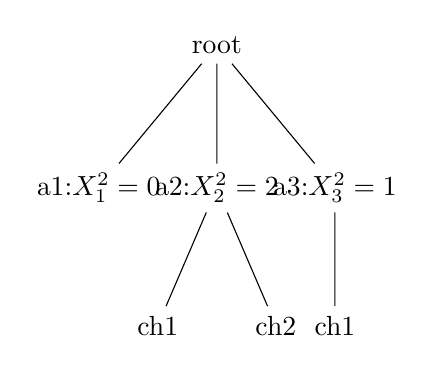
\begin{tikzpicture}
\tikzstyle{every node}=[anchor=north]
\node {root}
child { node {a1:$X_1^{2}=0$}
}		
child { node {a2:$X_2^2=2$}
	child { node {ch1}}
	child { node {ch2}}
}
child { node {a3:$X_3^2=1$}
child { node {ch1}}
};
\end{tikzpicture}

so here in the picture for example :\\ 
$Z_0=1 \leftarrow$ Z0 = generation 0 has 1 element\\ 
and $Z_1=3 = = X_{Z_0=1}^1=3 \leftarrow $ Z1 = generation 1 has 3 children  \\
and $Z_2=3 = X_{1}^2 + X_{2}^2 + X_{Z_1=3}^2 = 0 + 2 + 1 \leftarrow Z_2 $ = num children in  generation 2 = 3 children

\subsection{calculation}
\begin{itemize}

\item Distribution of \boxed{Z_n} obtained from generating $ \Rightarrow f_n(\theta)  =  E(\theta^{Z_n}) = \sum \theta^k \boxed{ P(Z_n=k) }$ \\
\item $ f_{n+1}(\theta) = E  \theta^{Z_{n+1} } = E \left(  \boxed{E\theta^{Z_{n+1}}|Z_n} \right) = \sum \boxed{E  \left( \theta^{Z_{n+1}} | Z_n    \right)}  P(Z_n=k) \leftarrow \boxed{E  \theta^{Z_{n+1}} | Z_n}     $ is the random variable here \\
\item so now standard calc : $E  \left( \theta^{Z_{n+1}} | Z_n    \right) = E  \left( \theta^{Z_{n+1}} | Z_n=k    \right) = E  \left( \theta^{X_1^{n+1} + .. X_{Zn=k}^{n+1}} | Z_n=k    \right) $ \\
\item but (a) num children contributed by animal m  to generation n+1 = $x_m^{n+1}$ = not dependent on other siblings $x_{...}^{n+1}$ in its own generation (n), or indeed num of such siblings = $Z_n$ , so complicated expression $E  \left( \theta^{X_1^{n+1} + .. X_{Zn=k}^{n+1}} | Z_n=k    \right) = $ same without the conditioning = absolute expectation = $E  \left( \theta^{X_1^{n+1} + .. X_{Zn=k}^{n+1}} \right)$\\
\item and moreover (b) the $X_{.}^{n+1}$ are independent and independent = multiply 
\item  so $E  \left( \theta^{X_1^{n+1} + .. X_{Zn=k}^{n+1}} \right) = E\theta^{X_1^{n+1}} ... E\theta^{X_{Zn=k}^{n+1}} $ and all the $X_i^j$ have same distribution and $E\theta^X=f(0)$ and since there are $Z_n=k$ of them = ${f(\theta)}^k$\\
\item so finally $E  \left( \theta^{Z_{n+1}} | Z_n    \right) = {f(\theta)}^{Z_n}$ \\
\item so tower property $E (...)  = E \theta^{Z_{n+1}} = E {f(\theta)}^{Z_n} = f_n(\theta) $ by definition see first line \\
\item so $ E \theta^{Z_{n+1}} = f_{n+1}(\theta) = E {f(\theta)}^{Z_n} = f_n( f(\theta)) = f_n \circ f (\theta)$ \\
\item so  $\boxed{f_{n+1}(\theta) = f_{n}(\theta)}$

\end{itemize}

\subsection{extinction}
\begin{itemize}
\item extinction  = zero children in some generation = $\pi_n = P(Zn=0) = fn(0) $ \\
\item $\pi_{n+!} = P(Z_{n+1}=0) = f_{n+1}(0)\leftarrow$ recall $f(\theta)=E(\theta^X) = \sum \theta^k P(X=k) = P(X=0) + \sum_{k=1} \theta^k P(X=k)$\\
\item so $\pi_{n+1}=f(\pi_n)$ and extinction = 0 eventually = $\pi=\uparrow \lim \pi_n$ and f continuous so $\boxed{\pi= f(\pi)}$ with  $f(1)=1 \quad f(0)=P(X=0) \quad \text{slope at 1}=f'(1)=E(X)=\mu \longleftarrow \boxed{f'(\theta)=E(X\theta^{X-1})}$ so $f'(1)=E(X)$ \\
\item if $\mu>1$ then extinction with prob $\pi=f(\pi)$ before hits 1 but if if $\mu<1$ then extinction only when hits 1

\end{itemize}


\subsection{martingale}

\begin{itemize}
\item $Z_{n+1}$ = num children in (n+1) generation only depends on $Z_{n} \leftarrow$ Markov \\
\item $E(\theta^{Z_{n+1}} | Z_n) = {f(\theta)}  ^ {Z_n} $ so differentiate wrt $\theta$\\
\item $E(Z_{n+1} \theta^{Z_{n+1}-1} | Z_n) = Z_n {f(\theta)}  ^ {Z_n-1} f'(\theta) $ \\
\item and with $\theta=1 \rightarrowtail E(Z_{n+1}|Z_n) = Z_n 1^{whatever} f'(1) = \mu Z_n $\\
\item so $E (Z_{n+1}|Z_n) = \mu Z_n \leftarrow $ not a martingale \\
\item set $M_n = \frac{Z_n}{\mu^{n}} \leftarrow $ is a martingale - deflated the Zn\\
\item $E( M_{n+1} |Z_n  )  =  E(  \frac{Z_{n+1}}{\mu^{n+1}} |Z_n  ) = \frac{1}{\mu^{n+1}} E(Z_{n+1}|Z_n) = \frac{1}{\mu^{n+1}} \mu Z_n= \frac{z_n}{\mu^{n}}= M_n $ \\
\item $E( M_{n+1} |Z_n  ) = M_n \leftarrow \mycondE{M_{n+1}}{Z_n} $ \textbf{M}n martingale relative to \underline{\textbf{Z}}n \\
\item $\myE{M_{n+1}} = \myE{M_n} = ... = \myE{M_0} = Z_0 = 1$ \\
\item \boxed{MCT} because Mn >= 0 $ \rightarrowtail \text{EXISTS ALMOST SURELY } M_{\infty} = \lim M_n = \lim \frac{Z_n}{\mu^n}$ \\
\item CAUTION $  \myE{M_n}=1 \quad \lim M_n = M_{\infty} \text{ exists but if } \mu<=1  \rightarrow = M_{\infty}=0 $ so sometimes $\myE{M_{\infty} = \lim M_n}=0 \ne \myE{M_n} =1 $ ie $\myE{lim } <> \lim \myE{.} $\\

\item \boxed{\text{HOWEVER FATOU IS TRUE}} $\myE{\liminf Y_n} <= \liminf \myE{Y_n}$ ie $\myE{\liminf M_n}=\myE{M_{\infty}} = E(0) = 0 <= \liminf \myE{M_n} = \liminf 1 = 1$\\

\item  see reminder picture about FATOU  E (lim inf ) < lim inf E (.) below\\
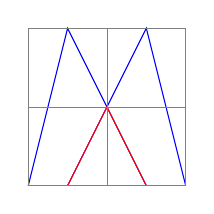
\begin{tikzpicture}
\draw  [blue]  (0,0) --(0.5,2) -- (1.5,0);
\draw  [blue]  (0.5,0) --(1.5,2) -- (2,0);
\draw  [red]  (0.5,0) --(1,1) -- (1.5,0);
\draw[help lines] (0,0) grid (2,2);
\end{tikzpicture}

\end{itemize}

\subsection{distribution of $\myMI$ }

\begin{itemize}
\item $\myMn \myeq {bct} {\rightarrow}  \myMI$ so $\exp(-\lambda \myMn) \rightarrow exp(-\lambda \myMI)$ \\
\item \boxed{BCT}  $ \myE{exp(-\lambda \frac{Z_n}{\mu^n})} < 1 \rightarrowtail$  $ \myE{exp(-\lambda \myMI)} = \myE{exp(-\lambda \lim \myMn)} \myeq{bct} \lim \myE{exp(-\lambda \myMn)} $ and $ \myE{exp(-\lambda \myMn)} = \myE{exp(-\lambda \frac{Z_n}{\mu^n})} = f_n \left(  \myexp{ \frac{-\lambda}{\mu^n}} \right)  $ \\
\item CONCLUSION $ \myE{exp(-\lambda \myMI)} \myeq{bct} \lim \myE{exp(-\lambda \myMn)} = \lim f_n \left(  \myexp{ \frac{-\lambda}{\mu^n}} \right) $
\end{itemize}

\subsection{ Now try a particular P(X=k) : $ P(X=k) = pq^k $ }
\begin{itemize}

\item $ P(X=k) = pq^k \Rightarrow f(\theta) = \myE{\theta^X} = \sum \limits_{k=0} \theta^k P(X=k) = \sum \limits_{k=0} \theta^k pq^k = \frac{p}{1-q\theta} \text{ ; and also } \mu = \frac{q}{p}$ \\

\item $ \pi = f( \pi ) \Rightarrow \pi = \frac{p}{1-q \pi} \Rightarrow (\pi=1 , \pi=\frac{p}{q} \iff \frac{p}{q} <1) $ \\

\item Need fn(theta) $ f(\theta) = \frac{p}{1-q\theta} \Rightarrow G = \mylp \begin{smallmatrix} a&b\\ c&d \end{smallmatrix} \myrp = \mylp \begin{smallmatrix} 0&p\\ 1& -q \end{smallmatrix} \myrp \Rightarrow G^n = {(SAS^{-1})}^{n} \Rightarrow f_n(\theta) = \frac{p \mu^n (1-\theta)+q\theta-p}{q \mu^n (1-\theta)+q\theta-p} $\\

\item $\mu <= 1 \Rightarrow \pi =1 \text{ (see earlier) and } \Rightarrow \lim f_n = 1 \Rightarrow \text{all in P(x=0)} \Rightarrow \text{process dies out}$ \\

\item $\mu > 1 \Rightarrow L(\lambda) = \myE{exp(-\lambda \myMI)} \myeq{bct} \lim \myE{exp(-\lambda \myMn)} = \lim f_n \left(  \myexp{ \frac{-\lambda}{\mu^n}} \right) \text{with fn as above it is found that } \Rightarrow L(\lambda) = \frac{p\lambda+q-p}{q\lambda+q-p} \myright{   Laplace   } L(\lambda) = \pi \myexp{- \lambda . 0 } + \int_{0}^{\infty} (1-\pi)^2 \myexp{-\lambda x} \myexp{-(1-\pi)x} dx \Rightarrow  
\begin{cases}
P(\myMI =0) = \pi  \\
P(x < \myMI < x+ dx) = (1-\pi)^2 \myexp{-(1-\pi)x} \Rightarrow P (\myMI > x) = (1-\pi)\myexp{-(1-\pi)x}
\end{cases} $

\item $\mu < 1 \Rightarrow $ process dies out (see above) but what is the distribution when it does not ie what is $ \myE{\theta^{Z_n} | Z_n \ne 0}$ ? It is $ \myE{\theta^{Z_n} | Z_n \ne 0} = \frac{f_n(\theta) - f_n(0)}{1-f_n(0)} \Leftarrow$ because recall $f_n(\theta)  =  E(\theta^{Z_n}) = \sum \theta^k P(Z_n=k) $ and we condition by dividing the intersection with the prob of the event $P(Z_n) \ne 0$

\item from above can show $\mu < 1 \Rightarrow \lim P(Z_n=k | Z_n \ne 0) = (1-\mu) \mu^{k-1}$ \\

\item So MYSTERY explanation as to why for  $\mu < 1 \Rightarrow \myE{M_n}=1$ but $\myE{\myMI} =0$ : for large n it turns out $ \myE{Z_n | Z_n \ne 0} = \sum k P(Z_n=k | Z_n \ne 0)  = \sum k (1-\mu) \mu^{k-1} = 1/(1-\mu) $ and (see above the intersection/division) $ P(Z_n) \ne 0 = 1 - f_n(0) = (1-\mu) \mu^n $ so $\myE{M_n} = \myE{M_n|Zn \ne 0} P(Z_n \ne 0) = \myE{\dfrac{Z_n}{\mu^n}|Z_n \ne 0} P(Z_n \ne 0) = \frac{1}{(1-\mu)\mu^n} (1-\mu) \mu^n =1$
\end{itemize}


\section{Chapter 1 - Measure spaces - sigma-algebra and pi-systems}

\begin{itemize}
	
\item algebra stable under finitely many  intersections / unions
\item $ A \cap B = \mylp A^c \cup B^c \myrp ^c $

\begin{venndiagram2sets}
	\fillACapB 
\end{venndiagram2sets}


\item $\sigma-$algebra stable under finitely many  interesections / unions
\item $ \cap A_n = \mylp \cup A^c \myrp ^c $
\item $ Borel (S) = B(S) = \sigma \text{(open sets in S)} $
\item $ Borel (\mathbb R) = B(\mathbb R) = \sigma \mylp \pi (R) \myrp $ where $ \pi(R) := \{ ( -\infty,x]  : x \in \mathbb R \} $
\item \colorbox{blue!10}{Proof} $\Leftarrow$  $ ( -\infty,x] = \cap_n   ( -\infty,x+1/n ) $ = countable intersections of open sets in B 
\item \colorbox{blue!10}{Proof} $\Rightarrow$ every borel is countable union of open intervals so sufficient to show for  $(a,b)$ and $(a,b) = \cup_n (a,b - \epsilon . 1/n \rbrack $ and $ (a, b \rbrack = ( -\infty , b \rbrack \cap (\infty,a)^c$
 
\item Additive measure $A \cap B = \emptyset \Rightarrow m (A \cup B ) = m(A)+m(B)$
\item Countably Additive measure $\text{disjoint sets } F_n  \Rightarrow m (\cup F_n ) = \sum m ( F_n) $
\item measure = countably additive $\Sigma -> \lbrack 0 , \infty \rbrack$
\item finite measure = $m (A) <\infty$   
\item $\sigma$-finite measure = there is a sequence $\cup F_n = S \text{ with } m (F_n) <\infty$ 
\item \textbf{Measure Extension theorem (Easy)} : 
\item $\pi\text{-system = family sets stable under finite intersection:} A,B \in I \rightarrow A \cap B \in I $
\item $m1(S)=m2(S) < \infty$ and $m1=m2$ on I $\Rightarrow$ $m1=m2 \text{ on } \Sigma$
\item \textbf{Measure Extension theorem (Corollary)} : 2 measures agree on pi-system -> agree on sigma algebra - and recall the case $B = B(R) = \sigma ( \pi (R))$    

\item \textbf{Measure Extension theorem (Caratheodory)} : countably additive function m0 on an algebra on set S can be extended to measure m on sigma (algebra) such that m0 = m on the algebra, and uniquely so if the measure is finite ie. m0 (S) < $\infty$

\item \textbf{Application: Lebesgue measure} collection $F= \cup \lbrack a_k, b_k \rbrack $ of sets on [0,1] with $m0(F) = \sum (b_k - a_k) $ and $ 0 \le a_1 \le b_1 \le ...bk \le 1 $ then m0 is additive, countably additive (not trivial -- see \colorbox{green!10}{proof}), and sigma (F) and $\sigma(F)=B(0,1\rbrack)$ (see \colorbox{blue!10}{proof} above) so now use extension theorem to extend and create Lebesgue measure.

\item \colorbox{green!10}{Proof sketch} : take collection Fn of disjoint elements with $F = \cup F_n$ and take $G_n = \cup_{k=1}^{k=n} F_n $ then obviously $G_n \uparrow F$ and $m0 (G_n) = \sum_1^n F_k$
\item  then just show that $ m0(Gn) \uparrow m0 (F) $ because then  $m0(F) := \uparrow \lim m0(Gn) = \uparrow \lim m0(\cup_{k=1}^{k=n} F_n) := m0(\cup_{k=1}^{k=\infty} F_n)$
\item  take $H_n = F \setminus G_n $ then $H_n \downarrow \emptyset$ so just show that $ m0(H_n) \downarrow 0 $
\item that is same as showing if $Hn \downarrow$ and $m0(H_n) > \epsilon \rightarrow \cap H_n \ne \emptyset$
\item to do that , take $ \overline{J_k} \subseteq H_k$ and $m0(H_k \setminus J_k) \le \epsilon 2^{-k}$ then $m0 ( H_n \setminus \cap_{k \le n} J_k ) \le m0 ( \cup_{k \le n} H_n \setminus  J_k ) \le \epsilon \sum 2^{-k} \le \epsilon$ so $mo \mylp \cap_{k \le n} J_k \myrp  \ge \epsilon $ 
\item so $ \cap_{k \le n} J_k \ne \emptyset$ so  $ K_n := \cap_{k \le n} \overline{J_k} \ne \emptyset$ so $ \cap_{k \le n} H_k \ne \emptyset$ 
\item finally it follows $ \cap \overline{J_k} \ne \emptyset$ because $\overline{J_k}$ is compact so choose a point inside $ K_n$ and find a subsequence that $\rightarrow $ inside the compact
\item \colorbox{green!10} {end of proof}
\item inequalities
\end{itemize}
\begin{mdframed}
$
\mu (A \cup B) \le \mu(A) + \mu(B)  \\
\mu (A \cup B) = \mu(A) + \mu(B) - \mu (A \cap B) \Leftarrow A \cup B =  A \cup (B \setminus \mylp A \cap B \myrp )\\
\mu (\cup_n U_i) \le \sum_n \mu (U_i)  \\
\mu (\cup_n U_i) = \sum_n \mu(U_i) - \sum \sum_{i<j} \mu(U_i \cap U_j) + \sum \sum \sum_{i<j<k} \mu(U_i \cap U_j \cap U_k) - ...   $  
\end{mdframed}

\begin{itemize}

\item \textbf{monotone convergence of measures - UP}
\end{itemize}
$
\boxed{F_n \uparrow F \Rightarrow \mu(F_n) \uparrow \mu(F)   \leftarrowtail F_n \uparrow F \text{ means } F_n \subseteq F_{n+1) \text{  and } \cup F_n = F} }$

\begin{itemize}

\item \colorbox{blue!10}{Proof} = $\mu(F_1 \cup \mylp F_2 \setminus F_1 \myrp \cup \mylp F_3 \setminus F_2 \myrp \cup F_n \setminus F_{n-1}  ) = \sum \mu (Fj \setminus F_{j-1}) = \sum_k \mu (G_k) \uparrow \sum_{\infty} \mu(G_k) = \mu(F)$


\item \textbf{monotone convergence of measures - DOWN - NEED FINITENESS}
\end{itemize}

\begin{mdframed}
$
F_n \downarrow F \text{  AND  } \mu(F_n) \text{  FINITE  } \Rightarrow \mu(F_n) \downarrow \mu(F)     $
\end{mdframed}

\begin{itemize} 
\item countable sum of null sets = 0
\item WARNING $ H_n = [ n,\infty ] \rightarrow H_n \downarrow \emptyset \quad \mu(H_n) = \infty$ 
\item WARNING : EXAMPLE of $\cap \cup I_{n,k} \neq \cup \cap I_{n,k}$  
\item  $ V = Q \cap [0,1] = [v_n] \text{ all rationals in [0,1] } \subseteq G_k = U_n [ v_n - \epsilon_k / 2^n , v_n + \epsilon_k / 2^n ] = \cup I_{n,k}$ with $\epsilon_k \downarrow 0 $ ie doubly infinite sum 
\item V = countable union = measure 0
\item H = $\cap G_k = \emptyset $ = measure 0 and obviously $ V \subseteq H$
\item however (not proved - Baire category theorem) H is \textbf{uncountable}
\item cannot have countable = uncountable 
\item so $ H = \cap G_k = \cap \cup I_{n,k} \neq \cup \cap I_{n,k} = V$
\item so careful interchanging things: 
\item END of WARNING 

\end{itemize}
	
\section{Chapter 2 - Events, $\limsup$ , $\liminf $}

\begin{itemize} 
\item $\Omega$ = sample space = set of outcomes, $\omega$ sample point = single outcome, $\mathcal{F} := \sigma$ -field on $\Omega$ is family of events

\item $\omega$ chosen 'at random' according to law $\mathbb{P}$, for $F \subseteq \mathcal{F} $ then $\mathbb{P} (F)$ = probability of F

\item Example coin toss F: = $ \bigg[ \omega : \dfrac{\# \mylp k \le n \quad  w_k=H \myrp}{n} \rightarrow \frac{1}{2} \bigg] $

\item almost surely : $F = \big[ \omega : S( \omega) = true \big] $ in $\mathcal{F}$ and has P(F) =1
\item $P(F_n)=1 \rightarrow P(\cap F_n) =1 \leftarrow P(F_n^c)=0 \Rightarrow P(\cup F_n^c) =0$ with $  {\big[\cup F_n^c\big]}^{c} = \cap F_n$

\item EXAMPLE / WARNING: $ F_{\alpha} = \bigg[ \omega : \dfrac{\# \mylp k \le n \quad  w_{\alpha(k)}=H \myrp}{n} \rightarrow \frac{1}{2} \bigg] \Rightarrow P(F_{\alpha})=1$ for all $ \alpha(k)$ sequences that go from $ 0 ... 1$ however $ \bigcap\limits_{\alpha \text{ sequences}} F_{\alpha} = \emptyset \leftarrowtail \forall \alpha \quad \exists \omega ...$

\item \colorbox{blue!10}{LIM SUP , LIM INF}

 $ \boxed { \limsup x_n := \inf_m \big( \sup_{n \ge m} x_n\big) = \downarrow \big( \sup_{n \ge m} x_n\big) } \leftarrow $  eventual inf of all the sups 
 \\
 $ \boxed { \liminf x_n := \sup_m \big( \inf_{n \ge m} x_n\big) = \uparrow \big( \inf_{n \ge m} x_n\big) } \leftarrow $  eventual sup  of all the infs



\pgfplotsset{compat=1.6}

\pgfplotsset{soldot/.style={color=blue,only marks,mark=*}} \pgfplotsset{holdot/.style={color=blue,fill=white,only marks,mark=*}}

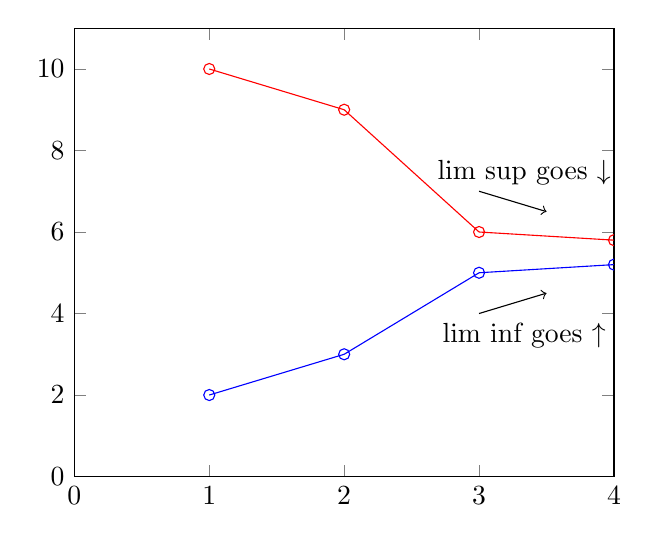
\begin{tikzpicture}
\begin{axis} [  xmin=-0, xmax=4, ymin=0,ymax=11]

\draw[red] (axis cs:1,10) circle[radius=2pt] -- (axis cs:2,9) circle[radius=2pt] -- (axis cs:3,6) circle[radius=2pt] -- (axis cs:4,5.8) circle[radius=2pt];

\draw[blue] (axis cs:1,2) circle[radius=2pt] -- (axis cs:2,3) circle[radius=2pt] -- (axis cs:3,5) circle[radius=2pt] -- (axis cs:4,5.2) circle[radius=2pt];

\node[anchor=north] (source) at (axis cs:3.3,8){ \text\ lim sup goes $\downarrow$};
\node[anchor=north] (source) at (axis cs:3.3,4){\text\ lim inf goes $\uparrow$ };

\draw[->] (axis cs:3, 4) -- (axis cs:3.5, 4.5);
\draw[->] (axis cs:3, 7) -- (axis cs:3.5, 6.5);

\end{axis}
\end{tikzpicture}

\item \colorbox{blue!10}{LIMIT} $\limsup = \liminf \leftarrowtail $ limits exists

\item \colorbox{blue!10}{LIM SUP , LIM INF - for SETS}

\item \item \colorbox{blue!10}{LIM SUP} 


\begin{enumerate}

\item $ E_n \text{ infinitely often}$ 
\item $:= \limsup E_n = \inf_m \big( \sup_{n \ge m} E_n\big)$
\item $=  \downarrow \big( \sup_{n \ge m} E_n\big) $
\item $=  \cap_{m} \cup_{n \ge m} E_n $
\item $= \forall m, \exists n(\omega) \ge m\text{ such that } \omega \in E_{n(\omega)} $
\end{enumerate}


\item  for each .., there exists ... $\rightarrow$ there is always one ... $\rightarrow$ infinitely often
\item  for each = $\cap$ , there exists = $\cup$

\item \colorbox{blue!10}{LIM INF}  

\begin{mdframed}[style=header]
$E_n \text{ eventually} := \\
 \liminf E_n = \sup_m \big( \inf_{n \ge m} E_n\big) \\
 = \uparrow \big( \inf_{n \ge m} E_n\big) \\ 
 = \cup_{m} \cap_{n \ge m} E_n \\
 =\text{ all the } m(\omega) \text{ that exist, such that every } n(\omega) \ge m(\omega) \text{ : } \omega \in E_{n(\omega)}$
\end{mdframed}


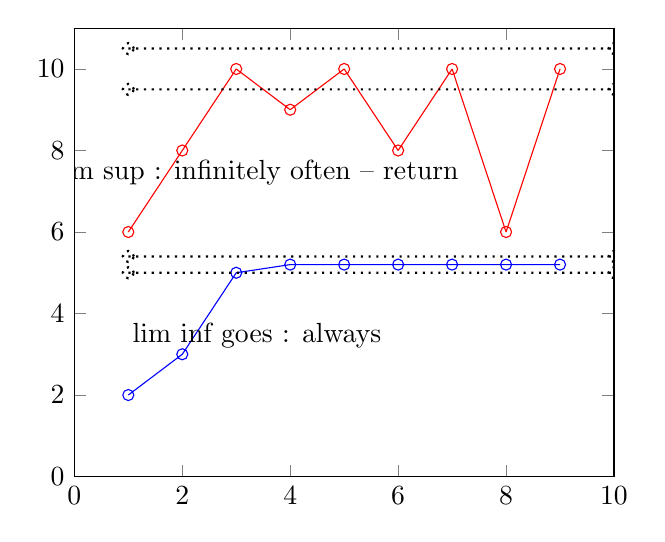
\begin{tikzpicture}
\begin{axis} [  xmin=-0, xmax=10, ymin=0,ymax=11]

\draw[red] (axis cs:1,6) circle[radius=2pt] -- (axis cs:2,8) circle[radius=2pt] -- (axis cs:3,10) circle[radius=2pt] -- (axis cs:4,9) circle[radius=2pt] -- (axis cs:5,10) circle[radius=2pt] -- (axis cs:6,8) circle[radius=2pt]-- (axis cs:7,10) circle[radius=2pt] -- (axis cs:8,6) circle[radius=2pt] -- (axis cs:9,10) circle[radius=2pt];

\draw[black,dotted,thick] (axis cs:1,9.5) circle[radius=2pt] -- (axis cs:10,9.5) circle[radius=2pt];

\draw[black,dotted,thick] (axis cs:1,10.5) circle[radius=2pt] -- (axis cs:10,10.5) circle[radius=2pt];

\node[anchor=north] (source) at (axis cs:3.3,8){ \text\ lim sup : infinitely often -- return};

\draw[blue] (axis cs:1,2) circle[radius=2pt] -- (axis cs:2,3) circle[radius=2pt] -- (axis cs:3,5) circle[radius=2pt] -- (axis cs:4,5.2) circle[radius=2pt] -- (axis cs:5,5.2) circle[radius=2pt] -- (axis cs:6,5.2) circle[radius=2pt] -- (axis cs:7,5.2) circle[radius=2pt] -- (axis cs:8,5.2) circle[radius=2pt] -- (axis cs:9,5.2) circle[radius=2pt];

\draw[black,dotted,thick] (axis cs:1,5) circle[radius=2pt] -- (axis cs:10,5) circle[radius=2pt];

\draw[black,dotted,thick] (axis cs:1,5.4) circle[radius=2pt] -- (axis cs:10,5.4) circle[radius=2pt];


\node[anchor=north] (source) at (axis cs:3.3,4){\text\ lim inf goes : always };


\end{axis}
\end{tikzpicture}



\item \colorbox{blue!10}{FATOU 1} $ \boxed{P( \limsup E_n) > \limsup P(E_n) }$

\item proof: $ G_m = \cup_{n \ge m} E_n \rightarrow G_m \downarrow \limsup E_n \rightarrow meas(G_m) \downarrow meas (\limsup E_n) \rightarrow P(G_m) \downarrow P(\limsup E_n) $ 
\item  and also $P(G_m) = P(\cup_{n \ge m} E_n) \rightarrow P(G_m) >= sup_{n >=m} P(E_n) \rightarrow P(G_m) \ge \downarrow \lim_m sup_{n >=m} P(E_n) := \limsup P(E_n) $
\item  so $\rightarrow P(\limsup E_n) \ge \limsup P(E_n)$

\item example: (x1,x2) sequence = (0,1),(1,0),(0,1),(1,0),.... then sum x1+x2 = 1 -> limsup sum =1 , but (limsup x1,limsup x2) = (1,1) -> sum(limsup) = 1+1 = 2 $ \rightarrowtail \limsup (sum) =1 <= sum (\limsup) = 2\rightarrowtail \limsup \int <= \int \limsup$


\item example: 
\item $ \boxed{meas( \limsup E_n) > \limsup meas(E_n) }$ 
\item  meas(max) > max (meas)

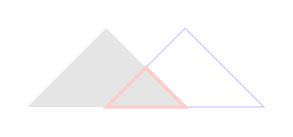
\begin{tikzpicture}

\fill[gray!20] (0,0) -- (1,1) -- (2,0) -- cycle;
\draw[blue!20] (1,0) -- (2,1) -- (3,0) -- cycle;
\draw[red!20,very thick] (1,0) -- (1.5,0.5) -- (2,0) -- cycle;

\end{tikzpicture}

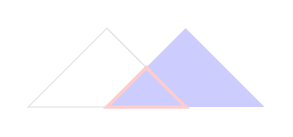
\begin{tikzpicture}

\fill[blue!20] (1,0) -- (2,1) -- (3,0) -- cycle;
\draw[gray!20] (0,0) -- (1,1) -- (2,0) -- cycle;
\draw[red!20,very thick] (1,0) -- (1.5,0.5) -- (2,0) -- cycle;

\end{tikzpicture}

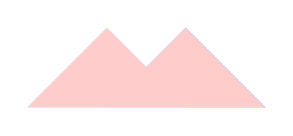
\begin{tikzpicture}

\draw[blue!20] (1,0) -- (2,1) -- (3,0) -- cycle;
\draw[gray!20] (0,0) -- (1,1) -- (2,0) -- cycle;
\fill[red!20] (0,0) -- (1,1) -- (1.5,0.5) -- (2,1) -- (3,0) -- cycle;

\end{tikzpicture}


\item \colorbox{blue!10}{BOREL-CANTELLI 1}  $ \boxed{\sum P(E_n) < \infty \rightarrow P(\limsup E_n) = 0 } \leftarrow$ limsup En is a set , and has a measure/prob and here prob/measure = 0. basically if the prob ifs finite -> things that happen i.o have prob 0 (logical!)

\item  proof: $P(G) <= P(G_m = \cup_{n \ge m} E_n) <= \sum_{n >= m} P(E_n)$

\item \colorbox{blue!10}{FATOU 2} $ \boxed{P( \liminf E_n) < \liminf P(E_n) }$

\item example: (x1,x2) sequence = (0,1),(1,0),(0,1),(1,0),.... then sum x1+x2 = 1 -> liminf sum =1 , but (liminf x1,liminf x2) = (0,0) -> sum(liminf) = 0+0 = 0 $ \rightarrowtail \liminf (sum) =1 >= sum (\liminf) =0 \rightarrowtail \liminf \int >= \int \liminf$
\item example: $f_n = \chi_{n,\infty} \longrightarrow \int \liminf f_n = 0 \le \liminf \int f_n = \infty$

\item hint: $\liminf x_n+\liminf y_n \le \liminf (x_n+y_n) \le \liminf x_n + \limsup y_n \le \limsup (x_n+y_n) \le \limsup x_n+\limsup y_n$ 
\item $ \boxed{meas( \liminf E_n) < \liminf meas(E_n) }$

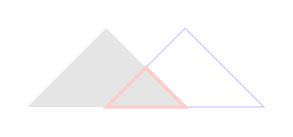
\begin{tikzpicture}

\fill[gray!20] (0,0) -- (1,1) -- (2,0) -- cycle;
\draw[blue!20] (1,0) -- (2,1) -- (3,0) -- cycle;
\draw[red!20,very thick] (1,0) -- (1.5,0.5) -- (2,0) -- cycle;

\end{tikzpicture}

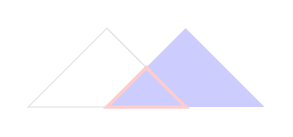
\begin{tikzpicture}

\fill[blue!20] (1,0) -- (2,1) -- (3,0) -- cycle;
\draw[gray!20] (0,0) -- (1,1) -- (2,0) -- cycle;
\draw[red!20,very thick] (1,0) -- (1.5,0.5) -- (2,0) -- cycle;

\end{tikzpicture}

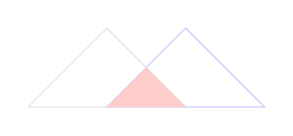
\begin{tikzpicture}

\draw[blue!20] (1,0) -- (2,1) -- (3,0) -- cycle;
\draw[gray!20] (0,0) -- (1,1) -- (2,0) -- cycle;
\fill[red!20] (1,0) -- (1.5,0.5) -- (2,0) -- cycle;

\end{tikzpicture}

\end{itemize}

\section{Chapter 3 - Random variables}

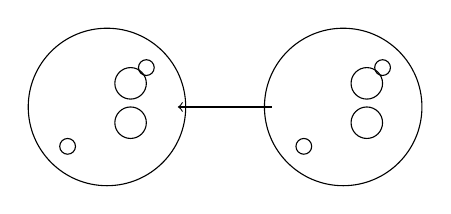
\begin{tikzpicture}

\draw  (3,3) circle [radius=1]; 
\draw  (3.5,3.5) circle [radius=0.1]; 
\draw  (3.3,3.3) circle [radius=0.2]; 
\draw  (3.3,2.8) circle [radius=0.2]; 
\draw  (2.5,2.5) circle [radius=0.1]; 

\draw [<-] (3.9,3) -- (5.1,3) ; 

\draw  (6,3) circle [radius=1]; 
\draw  (6.5,3.5) circle [radius=0.1]; 
\draw  (6.3,3.3) circle [radius=0.2]; 
\draw  (6.3,2.8) circle [radius=0.2]; 
\draw  (5.5,2.5) circle [radius=0.1]; 

\end{tikzpicture}

\begin{itemize}

\item note: sigma needed on target only!! f generates sigma on $\Omega \Leftrightarrow$ = sets generated by $f^{-1}$ on $\Omega$ from the target sigma. If there is a sigma on $\Omega$ as well, then measurability of f wrt that sigma-algebra $\Leftrightarrow$ sigma(f) $\in$ that sigma-algebra 

\item $ h := S \rightarrow \mathbb{R} \text{ measurable} \leftrightarrow h^{-1}(A) \in \Sigma \quad \forall A \in \text{Borel}$
\item $  h^{-1}(\cup A_{\alpha}) = \cup_{\alpha} h^{-1}(A_{\alpha}) \quad h^{-1}(A^c) = { \big[ h^{-1}(A) \big]}^c$
\item $ C \in B $ and $ \sigma(C) = B \rightarrow h^{-1} : C \rightarrow \Sigma \Rightarrow h \text{ measurable} $ Proof: take all element B such that $h^{-1}(B) \in \Sigma$, then these elements= $\sigma$ algebra in Borel by above, and $C \in B$
\item  $ \left\lbrace h <= s \right\rbrace \in \Sigma \Rightarrow h \text{ measurable}$ Proof: C = $\pi [-\infty,c]$ and $\sigma(C) = \mathbb{R}$ and use above
\item  sum and product and scaling of measurable = measurable Proof: eg for sum $ \{h1+h2 > c \} = \cup_{q \in Q} \{h1 > q\} \cap  \{h2 > c-q  \}  $ countable collection of $\Sigma$
\item   $ \boxed{ h_n \text{ measurable} \Rightarrow \inf h_n , \liminf h_n, \limsup h_n \text{measurable} } $ Proof: $ \{ \inf h_n > c \} = \cap_n \{ h_n > c \} $ , define $ L =\liminf h_n \quad L_n = \inf h_n   $ then $ \{ L < c \} = \cap_n  \{ L_n < c \}$
\item $ \boxed { \{ s : \lim h_n(s) \in \mathbb{R} \} \in \Sigma } $ Proof: the set = $ \limsup < + \infty \cap \liminf < - \infty \cap g^{-1} (0) $ where $ g := \limsup - \liminf $
\item  Strong law : $\Lambda = \{ \omega : \frac{\text{\#H}}{\text{\#tosses}} \rightarrow p \} = \{ \omega : L^+ (\omega) = p \} \cap \{ \omega : L^- (\omega) = p \} $ with L+ = limsup Sn/n , L- = liminf Sn/n where Sn = num Hs . n= num tosses


\item  \textbf{sigma-algebra on $\Omega$ generated by a sequence of functions} $ f_n : \Omega -> \mathbb{R}$= smallest sigma $\mathcal(E)$ on $\Omega$ such that every function in the sequence = measurable wrt that $\mathcal(E)$  ie $\sigma(f_n) = \sigma( \omega \subset \Omega : f_n(\omega) \in \mathcal{B})$

\item  Law of a random variable $L_X$:  
$$ \Omega \xrightarrow{X} \mathcal{R}$$
$$ [0,1] \xleftarrow {\mathbb{P}} \sigma(X) \text{  or  } \mathcal{F} \xleftarrow {X^{-1}} \mathcal{B} $$
$$ L_X = X^{-1} \circ \mathbb{P} : \mathcal{B} \rightarrow [0,1] $$
$$ F_X(c) := L_X [-\infty,c] = \mathbb{P} (X <= c) = P (\omega : X(\omega) <= c) $$ 
\item \textbf{distribution function $F_X$ is right continuous} : Proof: $P(X \le c+ \frac{1}{n}) \downarrow P(X \le c )$ because $F_n = G_n \setminus G_{n+1}$ with $G_n \downarrow G \rightarrow \mu(G_n) \downarrow \mu(G)$ because disjoint sets $\mu(G_1 \cup G_n) \uparrow \mu(G)$
\item variables with prescribed law (Skorokhod)

\begin{equation}
\begin{split}
X^+(\omega) & := inf (z : F(z)>w) = sup (y : F(y) \le \omega)\\
X^-(\omega) & := inf (z : F(z) \ge w) = sup (y : F(y) < \omega)\\
\end{split}
\end{equation}
\end{itemize}

\pgfplotsset{compat=1.6}

\pgfplotsset{soldot/.style={color=blue,only marks,mark=*}} \pgfplotsset{holdot/.style={color=blue,fill=white,only marks,mark=*}}

\begin{tikzpicture}[scale=0.5]
\begin{axis}
\addplot[domain=1.8:2,blue] {x*x};
\addplot[domain=2:2.2,blue] {x*x+1};
\draw[dotted] (axis cs:2,0) -- (axis cs:2,5);
\addplot[holdot] coordinates{(2,4)};
\addplot[soldot] coordinates{(2,5)};

\draw[dotted] (axis cs:0,4.5) -- (axis cs:2,4.5);

\draw[->] (axis cs:1.9, 1.9*1.9+0.1) -- (axis cs:1.95, 1.95*1.95+0.1);
\draw[<-] (axis cs:2.05, 1+2.05*2.05+0.1) -- (axis cs:2.1, 2.1*2.1+0.1+1);

\node[anchor=east] (source) at (axis cs:2.1,5){\text\ F(x)};
\node[anchor=east] (source) at (axis cs:1.95,3.5){\text\ F(x)};

\node[anchor=north](source) at (axis cs:1.8,4.6){$\omega$};
\node[anchor=south](source) at (axis cs:2,3.2){$X^{+/-}(\omega)$};

\node[anchor=north](source) at (axis cs:5,1){$$};

\end{axis}

\end{tikzpicture}

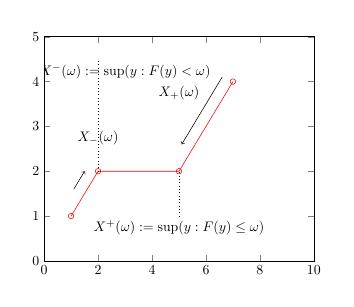
\begin{tikzpicture}[scale=0.5]

\begin{axis} [  xmin=-0, xmax=10, ymin=0,ymax=5]

\draw[red] (axis cs:1,1) circle[radius=2pt] -- (axis cs:2,2) circle[radius=2pt] -- (axis cs:5,2) circle[radius=2pt] -- (axis cs:7,4) circle[radius=2pt];

\draw[->] (axis cs:1.1, 1.1+0.5) -- (axis cs:1.5, 1.5+0.5);
\draw[->] (axis cs:6.1+0.5, 3.1+1) -- (axis cs:5.1, 2.1+0.5);

\node[anchor=north](source) at (axis cs:2,3){$X_-(\omega)$};
\node[anchor=north](source) at (axis cs:5,4){$X_+(\omega)$};

\node[anchor=north](source) at (axis cs:5,1){$X^+(\omega) := \sup (y:F(y) \le \omega)$};
\node[anchor=north](source) at (axis cs:3,4.5){$X^-(\omega) := \sup (y:F(y) < \omega)$};

\draw[dotted] (axis cs:2, 2) -- (axis cs:2, 4.5);
\draw[dotted] (axis cs:5, 1) -- (axis cs:5, 2);



\end{axis}


\end{tikzpicture}

\begin{itemize}

\item $X^-(\omega) = sup (y : F(y) \le \omega) $
\item so $\omega \le F(c) \Rightarrow X^-(\omega) \le c$ (1)
\item  $X^-(\omega) < c \rightarrow \omega \le F(c)$
\item  so $\omega \le F  (  X^-(\omega) ) $ because F right continuous
\item  so $X^-(\omega) \le c \Rightarrow \omega \le F  (  X^-(\omega) ) \le F(c) $ (2)
\item  so $X^-(\omega) \le c \Leftrightarrow \omega \le F(c)  $ (1)(2)
\item  so $X^-(\omega) \le c \Leftrightarrow \omega \le F(c)  $ (1)(2)
\item  so $ P (X^-(\omega) \le c)  = F(c)  $
\item   actually X+ and X- have same distiribution and $P (X+=X-) =1$ Proof: definition of X+ $\omega < F(c) \Rightarrow X^+(\omega) \le c$ so $F(c) \le P(X+ \le c)$ and X-<= X+ means $ (X+ \ne X-) = \cup_{q \in Q} X^- \le q \le X^+$ with $P (X- \le q \le X+) = P(X+ \le q) \setminus P(X- \le q) = F(q) - F(q) = 0$

\item \textbf{Sigma-algebras generated by collection of random variables} : observe the values $Y_{\gamma}(\omega) \Leftrightarrow$ observe $I_F(\omega)$ for $F \in \gamma = \sigma(Y_{\gamma}) \Leftrightarrow$ decide if F has occurred $\Leftrightarrow$ decide if $\omega \in F$ 
\item $\sigma(Y)$ for Y a r.v $=Y^{-1}(\text{Borel}) = \big\{\{w : Y(w) \in B \} \quad B \in \text{Borel} \big\}$
\item $Z : \Omega \rightarrow \mathbb{R}$ is sigma(Y)-measurable for some $Y : \Omega \rightarrow \mathbb{R}$ $\Leftrightarrow$ there is a Borel function $ f: \mathbb{R} \rightarrow \mathbb{R}$ such that Z=f(Y)
\item $Z : \Omega \rightarrow \mathbb{R}$ is sigma(Y1,Y2,..Yn)-measurable for some $Y_i : \Omega \rightarrow \mathbb{R}$ $\Leftrightarrow$ there is a Borel function on Rn $ f: \mathbb{R^n} \rightarrow \mathbb{R}$ such that Z=f(Y1,Y2,...,Yn)

\item $ Z : \Omega \rightarrow \mathbb{R}$ is sigma($Y_{\text{uncountable}}$)-measurable for some $Y_{\text{uncountable}} : \Omega \rightarrow \mathbb{R} \Leftrightarrow$  there is a Borel function on RN  $ f: \mathbb{R^N} \rightarrow \mathbb{R} $  such that Z=f $Y_{1},Y_{2},Y_{n}$ for some countable sequence inside the uncountable set. Note f of the form $\Pi_{uncountable} Borel(\mathbb{R})$ not $Borel(\mathbb{R}^{\text{uncountable}})$, the latter much bigger!

\item \textbf{MONOTONE CLASS THEOREM} $\pi$ systems $\rightarrow \sigma$ algebras $\Leftrightarrow$ indicator of elements of $\pi$ systems $\rightarrow$ general mesurable functions

\item \textbf{MONOTONE CLASS THEOREM} : $\mathcal{H}$ class of bounded functions $S \rightarrow \mathbb{R}$ such that 
\begin{enumerate}
\item $\mathcal{H}$ vector space
\item constant function 1 $\in \mathcal{H}$
\item if $f_n^+ \uparrow f$ and f bounded on S then $f \in \mathcal{H}$
\\then
\item indicator functions of $\pi$-system $ \mathcal{I} \in \mathcal{H} \rightarrow$ every bounded $\sigma ( \mathcal{I} )$-measurable function $\in \mathcal{H}$

\end{enumerate}

\end{itemize}

\section{Chapter 4 - Independence}



\begin{itemize} 

\item independent sigma algebras $\mathcal{G}_1,\mathcal{G}_2,\mathcal{G}_n$ $\Leftrightarrow$ $P(G_1,G_2,G_n)=P(G_1)P(G_2)P(G_n)$ for any $G_i \in \mathcal{G}_i$

\item independent variables = independent sigmas generated by the variables

\item independent events Ei $\Leftrightarrow$ the sigmas $\zeta_i=$ $\{\emptyset,E_i,\Omega,E_i^c=\Omega \setminus E_i\}$ independent = the rvs $I_{E_i}$ are independent and of course $\zeta_i=\sigma(I_{E_i})$
\item independent on Pi-system $\Leftrightarrow$ independent on sigma(pi system)

\item P(X<x,Y<y) = P(X<x)P(Y<y) $\Leftrightarrow$ pi-system(x),pi-system(y) independent $\Leftrightarrow$ the sigma(X),sigma() independents $\Leftrightarrow$ X,Y independents

\item \colorbox{blue!10}{BOREL-CANTELLI BC2IndepInf} : $E_n$ independent , $\sum P(E_n) = \infty \Rightarrow P(\limsup E_n)=1$

\item \colorbox{blue!10}{BOREL-CANTELLI BC1NoNeedLTI} : $ \sum P(E_n) < \infty \Rightarrow P(\limsup E_n) = 0 $ (recall - no need for independents)

\item \colorbox{blue!10}{BOREL-CANTELLI BC2IndepInf} : $E_n$ independent , $\sum P(E_n) = \infty \Rightarrow P(\limsup E_n)=1$ Proof: Compute and show $P \big\{ {(\limsup E_n)}^c \big\}=1$. With $ {(\limsup E_n)}^c = \liminf E_n^c = \cup_m \cap_{n \ge m} E_n^c$ and $P(\cap_{n \ge m} E_n^c)=\prod_{n \ge m} (1-p_n)$ becasue independent and limit $r\ge n \ge m \quad r \uparrow \infty$=ok because both sides monotone and $ \prod_{n \ge m} (1-p_n) \le \exp(-\sum p_n )=0$ isnce $1-x < \exp(-x)$

\item \colorbox{green!10}{Example} given Xn so that $P(X_n > x)=e^{-x}$ $\rightarrow P(X > \alpha \ln n) = e^{-\alpha \ln n}=n^{-\alpha} = \frac{1}{n^{\alpha}}$ so $\rightarrow P(X > \alpha \ln n \text{ for infinitely many n)} =$ 0 or 1 depending if $\alpha > 1, \alpha \le 1$ . So with $\alpha=1 , L := \limsup \frac{X_n}{n} \rightarrow P(L \ge 1) \ge P( \frac{X_n}{\ln n}  \ge 1 \text{ ,infinitely often} ) =1$ , but   $P(L>1+\frac{2}{k})=0$ because with $\alpha=1+\frac{1}{k}$ , $P(L>1+\frac{2}{k}) \le P \big\{ X_n > (1+\frac{1}{k}) \ln n, \text{infinitely often} \big\} =0 $ so P(L=1) =1. Also, you can repeat this : $P(X_n > \ln n + \alpha \ln \ln n) = \exp-(\ln n + \alpha \ln \ln n) = \frac{1}{n {(\ln n)}^{\alpha}} $ = same thing with $\alpha<=1 , > 1$ 

\item (cumulative) distribution function $P(X_n \le x) = F(x)$

\item sample path: $\omega \rightarrow X_n(\omega)$ 

\item \colorbox{green!10}{Monkey typing Shakespeare}. $H$=type infinitely many copies, $H_{k}$=type $\ge k$ copies, $H_{k,m}$=type $\ge k$ copies in [1,m], $H^{m}$ : infinite copies in $[m,\infty[$. independence between [1,m] and $[m,\infty[$ so $ P( H_{m.k} \cap H^m )= P (H_{m.k}) P (H^m) $, but (1) $H^m=H \quad \forall m$ (2) $H_{m,k} \uparrow H_m$ (3) $H_k \downarrow\ H$ so $ P( H_{m.k} \cap H^m )= P (H_{m.k}) P (H^m) \Rightarrow P(H \cap H) = P(H) = P(H) P(H) $ so P(H)=0,1 . (Actually  with BC2: P(H)=1 because if $P(X=x)=\epsilon$, so $E_n=$P(type Shakespeare immediately ie in [n..N+n]) $\ge \epsilon^N > 0$ so $\sum P(E_n)=\infty \Rightarrow P(\limsup E_n)=1$

\item Tail algebra of $\{X_n\}$ := $\tau := \cap {\tau}_n$ with ${\tau}_n=\sigma(X_n,X_{n+1},...)$

\item Tail algebra $\Tau$ has events like $F_1 := \{ \lim X_k \text{exists} \} = \{ \omega : \lim X_k(\omega) \text{ exists }  \}$ , $F_2 := \{ \sum X_k \text{ converges } \} $, $F_3 := \{ \lim \frac{\sum X_k}{n} \text{exists} \} $

\item rv measurable wrt Tail algebra $\Tau$ like $\zeta_1 = \limsup \frac{\sum X_k}{n}$

\item  \colorbox{green!10}{Example : proof that $F_3 \in \Tau$} $$F_3^n := \lim_k \frac{X_{n+1} (\omega)+X_{n+2} (\omega) +...+ X_{n+k} (\omega)}{k} : \omega \text{ exists }$$ then for every n, $F_3^n=F_3$. But the $X_n,X_{n+1},..$ are in the $\Tau_n$, so $F_3^n \in \Tau_n$

\item \textbf{Kolmogorov 0-1 law} : (A) $F \in \Tau \Rightarrow P(F)=0,1$ (B) for any rv $\eta \text{ on } \Tau$ , $P (\eta=c)=1$ for some $c \in [-\infty,+\infty]$ \textbf{ Proof (A) } let $\chi_n=\sigma(X_1.X_2...,X_n)$ and $\Tau_n=\sigma(X_{n+1}.X_{n+2}...)$ .Then \textbf{(1)} $\chi_n , \Tau_n$ are independent because pi-system $X_i<x_i$ generates $\chi_i$ and pi-system $X_j<x_j , n+1 \le j \le n+r, r \in \mathbf{N}$ generates $\Tau_n$ and these pi-systems are independents. \textbf{(2)} $\chi_n , \Tau$ are independent because $\Tau \in \Tau_n$ \textbf{(3)} $\chi_{\infty}:= \sigma(\chi_n),\Tau$ are independent because $\cup_n \chi_n$ is a pi-system since $ \chi_n \in \chi_{n+1} $ and it generates $\chi_{\infty}$ \textbf{(4)} $\Tau \in \chi_{\infty}$ \textbf{(5)} so $\Tau,\Tau$ independent ! \textbf{(6)} so $P(F) = P(F \cap F) = P(F) P(F) \quad \forall F \in \Tau$ \textbf{Proof (B)} just showed $P(\eta \le c)=0,1 \quad \forall c \in \mathbb{R}$ for any $\eta \in \Tau$ so at some poitn it goes 0 -> 1 so let $c=sup \bigg \{ x : \big \{ P (\eta <= x)  = 0 \big \}  \bigg  \} $ and then usual $P(\eta \le c-1/n ) =0$ $P(\eta \le c+1/n ) =1$ and $P(\cup)=0$ and $P(\cap)=1$ so P(=c)=1

\item \textbf{Note branching example} : $M_{\infty}$ is in tail alebra and not deterministic but then again the $Z_n$ are not independent

\item \colorbox{green!10}{Example} let $P(Y_i=-1)=P(Y_i=1)=\frac{1}{2} $ and let $X_n=Y_0Y_1...Y_n$. the $X_n$ are independent. Define $\Gamma=\sigma(X_1,X_2,...)$ and $\Tau_n=\sigma(X_n,X_{n+1},...)$. Then we can prove $\Lambda := \cap_n \sigma(\Tau_n,\Gamma) \neq \zeta := \sigma(\cap_n \Tau_n,\Gamma)$ \textbf{Proof}: $\Tau_0=\sigma(X_1,X_2,..),\Tau_1=\sigma(X_2,X_3,..),\Tau_{n-1}=\sigma(X_n,X_{n+1},..), Y_0=\frac{X_n}{Y_1Y_2...Y_n}$ so (a) $Y_0 \in \Gamma \text{ and also } \in \Tau_{n-1} \rightarrow Y_0 \in \Lambda := \cap_n \sigma (\Gamma,\Tau_{n-1})$ (b) if $\Pi=\cap$-stable then independence wrt $\Pi \Leftrightarrow $ sigma($\Pi$), and G:=$\cap_n \Tau_n \cap \Gamma$ is $\cap$-stable, and $Y_0$ independent of G because  $P\big \{ (Y_0 \in A) \cap g \big \} = P(Y_0 \in A)P(g),\forall A \in Borel,\forall g \in G$ because any g is $g=g_1 \cup g_2, g_1 \in \Gamma, g_2 \in \cap_n \Tau_{n-1}$ and $Y_0$ indep of $\Gamma$ and $P(g_2)=0,1$ since tail-algebra (Kolmogorov 0-1)

\end{itemize}

\section{Chapter 5 - Integration}
\begin{itemize}

\item notation : $\int_{\Omega} f d\mu = \mu (f,\Omega) = \mu (f) = \int_{\Omega} f(s) \mu(ds)$ and $\int_{A} f d\mu = \mu (f,A) = \int_{A} f(s) \mu(ds) = \mu(fI_A)$

\item +ve simple = +ve finite sum of indicator functions = $f+ = \sum_1^m a_k I_{A_k},A_k \in \Sigma, a_k \in [0, +\infty ]$ and $\mu(f+)=\sum a_k \mu(A_k)$, general $f \in m\Sigma+ \rightarrow \mu(f) = \sup \mu(simple), simple \le f$

\item \colorbox{red!10}{MON} $\boxed{ {f_n} \in m\Sigma+, f_n \uparrow f \Rightarrow \mu(f_n) \uparrow \mu(f) := \int_S f_n(s) \mu(ds) \uparrow \int_S f(s) \mu(ds) } \longleftarrow $ (Recall \colorbox{red!10}{MON for measure}  1.10.a: $F_n \in \Sigma, F_n \uparrow F \Rightarrow \mu(F_n) \uparrow \mu(F) \longleftarrow $ recall ($F_n \uparrow F$ means $F_n \in F_{n+1} , \cup F_n = F$)
\item for a given f. can build $f_n$ using staircase function $a^{(r)}=0,\frac{i-1}{2^r},r$ for $x=0,\frac{i-1}{2^r} < x \le \frac{i}{2^r} \le r (\ i \in \mathbf{N}) , x>r$ and set $f_n = a^{(n)} \circ f$ Note $a^{(r)}$ is left-continuous so (reverse) $f_n \uparrow f \Rightarrow a^{(r)}(f_n) \uparrow a^{(r)}(f)$

\item \colorbox{red!10}{MON A.E.} $\boxed{ {f_n} \in m\Sigma+, f_n \uparrow f \colorbox{red!30}{A.E.} \Rightarrow \mu(f_n) \uparrow \mu(f) }$ \textbf{Proof:} 

\item \colorbox{red!10}{FATOU - illi} $\boxed{   \mu (\liminf f_n) \le \liminf \mu(f_n) \ \forall f_n \in m\Sigma+ } \longleftarrow $ Recall: $\boxed{P( \liminf E_n) < \liminf P(E_n) }$ \textbf{Proof:} define $ g_k := \inf_{n \ge k} f_n \rightarrow \liminf_n f_n \myeq{(*)}: \uparrow \lim g_k, \forall n \ge k : f_n \ge g_k \rightarrow \mu(f_n) \ge \mu(g_k), \Rightarrow \mu(g_k)  \le \inf_{n \ge k} f_n $ so $ \mu (\liminf_n f_n) \myeq{(*)} \uparrow \lim_k \mu(g_k) \le \uparrow \lim_k \inf_{n \ge k} \mu(f_n) := \liminf_n \mu(f_n)$

\item  \colorbox{red!10}{FATOU2 -- needs a dominating FINITENESS $\mu(g)$} 
\end{itemize}
\begin{mdframed}

$f_n,g \in m\Sigma+, f_n \le g \forall n, \mu(g) < \infty \Rightarrow \mu(\limsup f_n) \ge \limsup \mu(f_n)$
\end{mdframed}

Proof: $h_n := g-f_n$ then FATOU1 $\mu(\liminf h_n) \le \liminf \mu(h_n) \rightarrow \mu \big \{ \liminf (g-f_n) \big \} \le \liminf \mu \big \{ (g-f_n) \big \} $ , now \textbf{$\limsup f_n = -\liminf (-f_n)$} so removing g (ok since finite): $\mu \big \{ \liminf (-f_n) \big \} \le \liminf \mu  (-f_n) \rightarrow  -\liminf \mu  (-f_n) \le \mu \big \{ -\liminf (-f_n) \big \} \rightarrow \limsup \mu (f_n) \le \mu \big \{ \limsup f_n \big \}$

\begin{itemize}

\item $f \in m\Sigma, f = f^+ - f^- := \max (f,0) - \max (-f,0), |f|=f^+ + f^-$ with $f^+,f^- \in m\Sigma^+$

\item  \colorbox{green!10}{INTEGRABLE} for $f \in m\Sigma$, f is $\mu$-integrable $:= f \in \mathbb{L}^1 (S,\Sigma,\mu) $ if $\mu(|f|) = \mu(f^+) + \mu(f^-) < \infty$, and then we set $\int f d\mu = \mu(f^+) - \mu(f^-)$

\item  $ |\mu(f)| \le \mu(|f|) $ like FATOU2

\item  \colorbox{red!10}{DOM - $L^1$ convergence}
\begin{enumerate}
\item $ f_n,f \in m\Sigma$
\item $f_n(s) ->  f(s)$
\item $|f_n(s)| \le g(s) \ \forall s \in S, n \in \mathbf{N}$
\item $\mu(g) < \infty$

\item then  $\Rightarrow f_n \rightarrow f \text{ in } L^1 (S,\Sigma,\mu) $ 
\item ie $\mu \big \{ |f_n - f| \big \} \rightarrow 0$ 
\item  note therefore $\mu(f_n) \rightarrow \mu(f)  $  
\end{enumerate}

\textbf{Proof:} $|f_n - f| \le 2g , \mu(g) < \infty \myright{FATOU2} \limsup \mu |f_n -f| \le \mu \big \{ \limsup |f_n -f| \big \} = \mu(0) = 0 \leftarrow |\mu(f_n) -\mu(f)| = | \mu(f_n-f)| \le \mu |f_n -f| $ 

\item  \colorbox{red!10}{SCHEFFE} $ f_n,f \in L^{1,+}, f_n \rightarrow f$ a.e then $\mu |f_n-f| \rightarrow 0  \Leftrightarrow \mu(f_n) \rightarrow \mu(f)$ \textbf{Proof $\looparrowright$} $ |\mu(f_n-f)| \le \mu|f_n-f| \rightarrow 0$ so done. \textbf{Proof} $\looparrowleft$ so suppose $\mu(f_n) \rightarrow \mu(f)$ and by hyp $f_n \rightarrow f$ then (a) $because (f_n-f)^- \le f \myright{DOM} \mu \big \{ {(f_n-f)}^- \big \}\rightarrow 0$ (b) \( \mu \myblp {(f_n-f) }^+ \mybrp = \mu  (f_n-f;f_n \ge f) = \mu(f_n-f) - \mu(f_n-f;f_n<f) \) and $  | \mu(f_n-f;f_n<f) | \le \ \mu{(f_n-f)}^- \rightarrow 0 $

\item standard machine: prove for indicator, prove by linearity  for SF+ = finsite sum, use (MON) for $m\Sigma+$, set $h=h^+ - h^-$

\item $ f \in m\Sigma^+, (f\mu)(A) := \mu(f;A) := \mu(fI_A)$ and $f\mu$ is  measure.
\item $\big \{ h(f\mu) \big \} (A) := (f\mu)(hI_A) =\mu \{ fhI_A \} = \big \{ hf(\mu) \big \} (A) $
\item \colorbox{red!10}{RADON-NIKODYM} $\mu,\lambda\ \sigma\text{-finite on } (S,\Sigma) $ then if $\mu(f)=0 \rightarrow \lambda(F)=0\ \forall F \Rightarrow \lambda = f\mu$ for some $f \in m\Sigma^+$

\end{itemize}

\section{Chapter 6 - Expectation}

\begin{itemize}
\item $E(X) := \int_{\Omega} XdP = \int_{\Omega} X(\omega) P(d\omega)$ for $X \in L^1=L^1(\Omega,F,P)$

\begin{enumerate}
\item if $X_n,X$ are such that $X_n \myright{a.s.} X$ ie $P(X_n \rightarrow X)=1$

\item \colorbox{green!10}{MON-Prob $ \boxed{ 0 \le X_n \uparrow X \Rightarrow E(X_n) \uparrow E(X) \le \infty }$ } $ \hookleftarrow {f_n} \in m\Sigma+, f_n \uparrow f \Rightarrow \mu(f_n) \uparrow \mu(f) := \int_S f_n(s) \mu(ds) \uparrow \int_S f(s) \mu(ds) $

\item \colorbox{green!10}{FATOU-Prob $ \boxed { X_n \ge 0 \Rightarrow E(X) \le \liminf E(X_n) }$ } $ \hookleftarrow \mu (\liminf f_n) \le \liminf \mu(f_n) \ \forall f_n \in m\Sigma+$

\item \colorbox{green!10}{DOM-Prob $ \boxed { |X_n(\omega)| \le Y(\omega), E(Y) < \infty \Rightarrow E|x_n-X|\rightarrow 0 }$ } $ \hookleftarrow $ see long one above

\item \colorbox{green!10}{SCHEFFE - Prob $  \boxed{ E |X_n| \rightarrow E|X| \Rightarrow E|X_n-X|=0 }$ } $ \hookleftarrow f_n,f \in L^{1,+}, f_n \rightarrow f$ a.e then $\mu |f_n-f| \rightarrow 0 \Leftrightarrow \mu(f_n) \rightarrow \mu(f) $

\item \colorbox{green!10}{BDD-DOMK $ \boxed{ |X_n(\omega)| \le K \Rightarrow E |X_n-X| \rightarrow 0 }$ } $ \hookleftarrow$ Note $E(K) < \infty$ because $P(\Omega)=1$

\end{enumerate}


\item notation $E(X,F) := \int_F X(\omega) P(d\omega) := E(XI_F)$
\item \colorbox{orange!10}{MARKOV} 

\begin{enumerate}
\item $  Z \in mF, g (nondec): \mathbb{R}->[0,\infty]\ Borel$
\item then $g \circ Z \in mF+$ and so 
\item $\Rightarrow \boxed { E(gZ) \ge E (gZ;Z \ge c) \ge g(c) P(Z \ge c) }$  $ \hookleftarrow$ examples $Z \in MF+, g(x) = x \Rightarrow E(gZ)=E(Z)  \ge c P(Z \ge c)$ , another example $X \in L1$ so $|X|$ as in first example, so $ E(|X|) \ge c P(|X| \ge c) $, final example $g(x)= e^{\theta x}, \theta \ge 0$ applied to $E(g(Z)) \ge g(c) P(Z \ge c) \Leftrightarrow \frac{E(g(Z))}{g(c)} \ge P(Y \ge c) $ is $ e^{-\theta c}E(e^{\theta Y}) \ge P(Y \ge c)$ $\looparrowleft$ choose a good c !
\end{enumerate}

\item useful results to remember
\begin{enumerate}

\item $X \in mF+, E(X) < \infty$ ie integrable , then obviously $P(X < \infty) =1 \looparrowleft$ remember Markov above $X \in mF+, P(Z \ge c) \le \frac{E(Z)}{c} $

\item $Z_k \in mF+$ then $E(\sum Z_k) \myeq{linear} \sum E(Z_k) \myle{MON} \infty$

\item $Z_k \in mF+$ with $E(\sum Z_k) < \infty \Rightarrow \sum Z_k < \infty$ (a.s) and therefore $\Rightarrow Z_k \rightarrow 0$ (a.s) $\twoheadleftarrow$ use the above 2 items
\item note : \colorbox{green!10}{BOREL-CANTELLI BC1NoNeedLTI : } \colorbox{red!10}{$ \sum P(E_n) < \infty \Rightarrow P(\limsup E_n) = 0 $} is in fact due to the above: let $F_k$ such that $\sum P(F_k) < \infty$ and let $Z_k=I_{F_k}$, then $E(Z_k)=P(F_k)$ ( $ \looparrowleft E(1_A)=P(A)$ by definition!) and $\sum I_{F_k}$ = number of $F_k$ which occur

\end{enumerate}

\item \colorbox{green!10}{CONVEX} c convex: $c(px+qy) \le pc(x) + q c(y)$ with $0 \le p=1-q \le 1$ example $x^2,|x|,e^{\theta x}\ \theta \in \mathbb{R}$ and any function $c^{''} \ge 0$

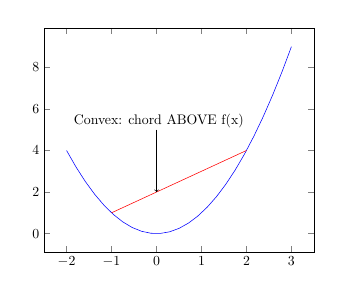
\begin{tikzpicture}[scale=0.5]
\begin{axis}
\addplot[domain=-2:3,blue] {x*x};
\addplot[domain=-1:2,red] {x+2};
\node[anchor=north] (source) at (axis cs:0,6){\text\ Convex: chord ABOVE f(x)};
\draw[->] (axis cs: 0,5) -- (axis cs: 0,2) ;
\end{axis}
\end{tikzpicture}

\item \colorbox{green!10}{JENSEN}
\begin{enumerate}
\item $ c: G \rightarrow \mathbb{R}$ 
\item $E|X| < \infty$
\item $P(X \in G)=1$
\item $E |c(X)| < \infty$
\item then \colorbox{green!10}{ $\Rightarrow c(E(X)) \le E(c(X))$} intuition $\looparrowleft c(px+qy) \le pc(x) + q c(y) $ so $\looparrowleft c(p_1 x_1+ p_2 x_2 + .. p_n x_n) \le p_1 c(x_1) + p_2 c(x_2) + ... + p_n c(x_n) $
\item Proof: c convex $\Delta_{u,v}=\frac{c(v)-c(u)}{v-u}$ so $\Delta_{u,v} \le \Delta_{v,w}$ so $\uparrow \lim_{u \uparrow v} \Delta_{u,v} = D^-(v)\le D^+(v) = \downarrow  \lim_{w \downarrow v} \Delta_{v,w}$ so for $m \in [D^-(v),D^+(v)]$ then $c(x) \ge m(x-v) + c(v),\ \forall x \in G$, in particular $v=\mu=E(x) \in G$ and substitute $x \rightarrow X$ (a.s) $c(X) \ge m(X-\mu) + c(v)$ and take E(.) then $E (c(X)) \ge m (E(x)-\mu)+c(\mu)$
\end{enumerate}

\item \textbf{Norm} : \colorbox{green!10}{ ${||Y||}_p = {E({|Y|}^p)}^{1 \over p}$ } for $E(|X|^p) < \infty$
\item \colorbox{green!10}{monotone $L^p$ $|| Y_p || \le || Y_r || $ with $1 \le p \le r < \infty $} \textbf{Proof:} use truncation to make bounded $X_n(\omega)= \big\{|Y(\omega)| \wedge n \big \}^p$ , bounded so $X_n , X_n^{r \over p}\in L^1$, use convex $c(x)=x^{r \over p}$ and JENSEN $c(E(X)) \le E(c(X))$ so $ {\{ E(X_n) \} }^{r \over p} \le E(X_n^{r \over p}) = E \big\{ {(|Y(\omega)| \wedge n)}^{r} \big \}$ which is $\le {\big \{ E {|Y|} \big \} }^r$ , so $E(X_n) ^ {1 \over p} \le {E {|Y|}^r }^{1 \over r} = ||Y_r||$ but (a) (MON) $X_n \uparrow Y^p$ so $E(X_n) \uparrow E(|Y|^p)$ so $E(X_n)^ {1 \over p} \uparrow {E(Y^p)}^{1 \over p} =  {||Y||}_p $ so ${||Y||}_p \le {||Y||}_r$

\item \colorbox{green!10}{\textbf{SCHWARTZ} $|E(XY)| \le E(|XY|) \le {||X||}_2 {||Y||}_2 $} Proof by truncation : let  $X_n = X \wedge n$ and $Y_n = Y \wedge n$ and $0 \le E \big \{ {(aX_n+bY_n)}^2 \big \} \ge 0 $ ie $E(a^2X_n^2 +2abX_nY_n + b^2Y_n^2) \ge 0$ with the $B^2-4AC<0$ (since no solution) so $ { \{ 2E(X_nY_n) \} } ^2 < 4 {E(X_n)}^2{E(Y_n)}^2 < 4 {E(X)}^2{E(Y)}^2$ and then let $n \uparrow \infty$ with MON like before

\item \textbf{Variance/Covariance }

\begin{enumerate}
\item $VAR=E\big \{ (X-\mu_X)(X-\mu_X)\big \}=COVAR(X,X)$
\item $COVAR(X,Y)=E \big \{(X-\mu_X)(Y-\mu_Y) \big \}$
\item $<X,Y>=E(XY)$
\item  correl = $cos \theta = \frac{<U,V>}{ {||U||}_2 {||V||}_2 }$
\end{enumerate}

\item \textbf{Completeness of $L^p$ : } 
\begin{enumerate}
\item $L^p$ is complete (Cauchy series converge and limit inside) 
\item $X_n$ Cauchy sequence in $L^p$ $\Leftrightarrow \sup_{r,s \ge k} {||X_r - X_s||}_p \rightarrow 0$
\item $X_n$ Cauchy sequence $\Leftrightarrow \exists X \in L^p\ \wasytherefore\ X_n \rightarrow X \in L^p$ ie ${||X_r -X ||}_p \rightarrow 0$
\item Proof: choose sequence ${||X_{\alpha_{n+1}} - X_{\alpha_n}||}_p < 2^{-n}$ then with p=1 and monotonocity $E|X_{\alpha_{n+1}} - X_{\alpha_n}| = {|| X_{\alpha_{n+1}} - X_{\alpha_n} ||}_1 \le {|| X_{\alpha_{n+1}} - X_{\alpha_n} ||}_p $ so $E \sum |X_{\alpha_{n+1}} - X_{\alpha_n}| < \infty$ , so $\sum \big \{ X_{\alpha_{n+1}} - X_{\alpha_{n}} \big \}$ converge almost surely (absolutely in fact), so $X_{\alpha_n}(\omega)$ converges, then set $X = \limsup X_n$ , so X is measurable and $X_{\alpha_n}\rightarrow X$. Then this X is the one to use for Lp completeness : for $r > \alpha_{n}$ we have  $E(|X_r-X_{\alpha_{t}}|^p) = {|| X_r - X_{\alpha_{t}} || }_p^p \le 2^{-np}$ for some $t \ge n$ and $r \ge \alpha_{t} $ . Then with Fatout ('illi') : $\mathbb{E}(|X_r-X|^p)\leq \liminf_{t\to\infty}\mathbb{E}(|X_r-X_{k_t}|^p)\leq 2^{-np}$, so $X_r-X$ in $L^p$ ,  so  X in $L^p$ since $L^p$ is a vector space and  $X_r \rightarrow X$


\end{enumerate}

\item \textbf{Law of a rv} \colorbox{green!10}{$\Lambda_X(B)=P(X \in B)$ }

\item $Eh(X)=\Lambda_X(h)=\int_{\mathbb{R}} h(x) \Lambda_X(dx)$, with $h=1_B$ , this is a definition ie  $Eh(X)=E1_B=P(X \in B)=\Lambda_X(B)= \int_{\mathbb{R}} 1_B(x) \Lambda_X(dx) = \int_{B} \Lambda_X(dx)$

\item \textbf{PDF of a rv} there is an $f$ such that $P(X \in B) = \int_B f_X(x) dx$ with $dx$ meaning $Leb(dx)$ and $\frac{d\Lambda_X}{dLeb} = f_X$

\item \colorbox{green!10}{H\"{O}LDER (p,q,mult)} let $ p,q > 1, \frac{1}{p} + \frac{1}{q} =1 , f \in m\Sigma, f \in L^p, h \in L^q, \mu({|f|}^p) = {||f||}_p^p < \infty$ then \colorbox{green!10}{ $|\mu(fh)| \le \mu(|fh|) \le {||f||}_p {||h||}_q$} \textbf{Proof} say $f,h \ge 0, \mu(f^p)>0$ then define a prob measure  $P=\frac{f^p\mu}{\mu(f^p)}$ [ $\looparrowleft$ recall $\mu(f^p) := \mu(f^p,\Omega) = \int_{\Omega}f^pd\mu$ and also recall $f^p\mu$ is a measure ie $(f^p\mu)(A) := \mu(f^p;A)=\int_{A}f^p d\mu$ so that the division normalises to =1 ] , now use  $u(s) := \frac{h(s)}{ {f(s)}^{p-1}},f(s)>0; 0 $ otherwise, then because ${P(u)}^q \le P(u^q)$ [ $\looparrowleft$ recall JENSEN $c(E(X)) \le E(c(x))$ with $c(x) = x^q $ convex since $q >1$ ] , then $\mu(|fh|) \le {||f||}_p {||hI_{f>0}||}_q \le {||f||}_p {||h||}_q$ 
\item \textbf{Intuition} Holder (p=q=2) = Cauchy schwartz . Holder = $\|fg\|_1\le\|f\|_p\|g\|_p$ Cauchy = $\|fg\|_1\le\|f\|_2\|g\|_2$ ie $\left(\int fg\right)^2\leqslant\int f^2\cdot\int g^2$ and norm $ \int g^q=\|g\|_q^q,\quad \int f^p=\|f\|_p^p,\quad \int fg=\|fg\|_1 $

\item \colorbox{green!10}{H\"{O}LDER $|E(XY)| \le E(|XY|) \le {E({|X|}^p)}^{1 \over p} {E({|X|}^q)}^{1 \over q}$} Proof : $Q(\Lambda) =  \frac{E(1_{\Lambda}X^p)}{C=E(X^p)} $ , $Z=\frac{Y}{X^{p-1}}1_{X>0} , {(E_Q(Z))}^q \le E(Z^q) $ then $ {1\over {C^q}} E{(XY)}^q = {1\over {C^q}} E{(Y X^{1-p} X^{p} )}^q = {(E_Q(YX^{1-p}))}^q \myle{JENSEN} E_Q( {(YX^{1-p})}^q) = {1 \over C} E ( {(YX^{1-p})}^q X^p) = {1 \over C} E ( Y^q X^{q(1-p)}X^p) = {1 \over C} E(Y^q X^{-p} X^p) = {1 \over C} E(Y^p) $ so ${(E(XY))}^q \le C^{q-1} E(Y^q)$ so $E(XY) \le C^{ {q-1} \over {q}} {E(Y^q)}^{ 1 \over q} = C ^{1 \over p} {E(Y^q)}^{ 1 \over q} =  {E(X^p)}^{ 1 \over p} {E(Y^q)}^{ 1 \over q}  $

\item \colorbox{green!10}{MINKOWSKI (p,sum,triangle) ${||f+g||}_p \le {||f||}_p + {||g||}_p  $ } with $f,g \in L^p$ \textbf{Proof} use Holder $\mu({|f+g|}^p) = \mu({|f+g|}^{p-1}|f+g|) \le \mu({|f+g|}^{p-1}|f|) +  \mu({|f+g|}^{p-1}|g|) \myle{JENSENx2} {||f||}_p \quad {||\ {|f+g|}^{q-1}\  ||}_q + {||g||}_p \quad {||\ {|f+g|}^{q-1}\  ||}_q $ 

\end{itemize}

\section{Chapter 7 - Easy strong law}

\begin{itemize}

\item \textbf{Independence=Multiply} $E(XY)=E(X)E(Y)$ \textbf{Proof}: use staircase function [ $\looparrowleft$ Recall  $a^{(r)}=0,\frac{i-1}{2^r},r$ for $x=0,\frac{i-1}{2^r} < x \le \frac{i}{2^r} \le r (\ i \in \mathbf{N}) , x>r$ ] and set $ f^{(r)}=a^{(r)} \circ f \uparrow f (MON)$ on disjoint partitions and $a^{(r)}(X)=\sum a_i I_{A_i} , a^{(r)}(Y)=\sum b_i I_{B_i} $ on $A_i,B_i \in \sigma(X),\sigma(Y)$ and $P(A_i \cap B_i)=P(A_i)P(B_i)$

\item \textbf{Independence} $\operatorname{Cov}(XY)=0$ and $\operatorname{Var}(X+Y)=0$

\item \textbf{Strong Law - simple form - 4th moments -avg=0} $X_1,X_2...$ indeps, $E(X_i)=0,E(X_i^4)\le K \Rightarrow \text{ let } S_n=X_1+..+X_n \text{ then } P( \frac{S_n}{n}\rightarrow 0)=1$ ie $\frac{S_n}{n} \rightarrow 0 \text{ a.s}$ $\looparrowleft$ note the average is 0 in this form here. \textbf{Proof} terms with single $X_(.)^1$ ie $E(X_iX_j^2X_k)=E(X_iX_j^3)=E(X_iX_jX_kX_l)=0$ with indep and $E(X_i)=0$, terms like $E(X_i^2X_j^2)=E(X_i^2)E(X_j^2) \le K$ because $ {E(X_i^2)}^2 \myle{Jensen} E(X_i^4) \le K$ so $E(S_n^4)=E( {(X_1+..X_n)}^4 )=E(\sum_k X_k^4 + 6 \sum\sum_{i<j} X_i^2X_j^2) \le nK + 6\frac{n(n\colorbox{green!10}{-}1)}{2}K \le 3Kn^2$ and these are sums of +ve rvs so $E(\sum {(\frac{S_n}{n})}^4 ) \le 3K \sum {1 \over {n^2}} < \infty$ so (again see sum of +ve rvs) $\sum {(\frac{S_n}{n})}^4 < \infty \text{ a.s} \Rightarrow {S_n \over n} \rightarrow 0 \text{ a.s}$

\item \colorbox{green!10}{\textbf{Chebyshev} $P(|X-\mu| >c) \le {\operatorname{Var}(X) \over {c^2}} $} \textbf{Proof} $P(|X-\mu| > c) = P( {(X-\mu)}^2 > c^2) \myle{markov} {{E{ (X-\mu)}^2) } \over {c^2}}$ \textbf{Example} Bernoulli $P(X_i=1)=p, P(X_i=0)=1-p$ then $E(X_i)=1.p+0.(1-p)=p$ and $\Var(X_i)=E({X_i}^2)-E(X_i)^2=p-p^2=p(1-p)$ so $E(S_n)=np,\Var(S_n) \myeq{indep.} \sum \Var(X_i)=np(1-p) \le n/4 $ so $E(S_n/n)=p, \Var({S_n \over n})={\Var{S_n} \over {n^2}} \le {1 \over {4n}} $ so \textbf{Chebyshev} $P(| {S_n \over n}-p|>c) \le { 1 \over {4nc^2} } $ 

\item \textbf{Example Weierstrass polynomial} \colorbox{green!10}{$\sup_{s \in [0,1]} |B(x)-f(x)| \le \epsilon$} for some B polynomial, given f \textbf{uniformly} continuous [0,1] \textbf{Proof} $P(S_n=k)=\binom{n}{k}p^k (1-p)^{n-k}$ so define $B_n(x), x\in [0,1]$  by $B_n(p) := Ef( {S_n\over n})=\sum_0^n f({k \over n}) \binom{n}{k}p^k (1-p)^{n-k} $ then $|B_n(p)-f(p)|=|E{f({S_n \over n})-f(p)}| \myle{\colorbox{green!10}{jensen}} E(Y_n := |f({S_n \over n})-f(p)|)$ with $Z_n := {S_n \over n} -p$ then $Z_n$ small $\rightarrow Y_n$ small and $E(Y_n)= E(Y_n;Z_n \le \delta) + E(Y_n;Z_n > \delta) \le \text{small x }P(Z_n \le \delta) + 2K P(Z_n > \delta) \myle {see above} \text{small x }P(Z_n \le \delta) + 2K {1 \over {4n\delta^2}} $ ie small for n big enough.

\end{itemize}

\section{Chapter 8 - Product measures}

\begin{itemize}
\item MONOTONE CLASS THEOREM : H is a CLASS OF BOUNDED FUNCTIONS such that
\begin{enumerate}
\item H is a vector space
\item 1 is in H
\item $f_n^+$ is such that $f_n^+ \uparrow f$ then $f \in H \looparrowleft$ H closed under increasing limits of +ve  functions
\end{enumerate}
THEN
\begin{enumerate}[resume]
\item H contains the $I_x$ of all sets a pi-system on (S)  $\Rightarrow$ H contains all bounded  $\sigma-$(pi -system) measurable functions on S
\end{enumerate}


\end{itemize}

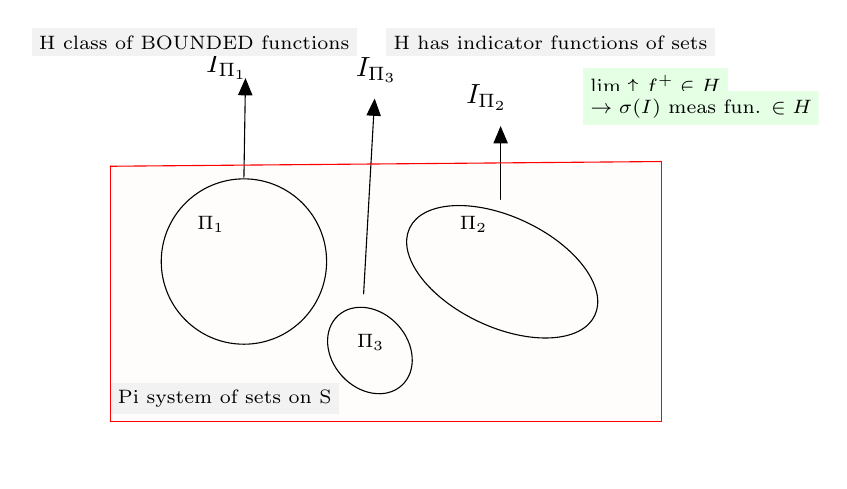
\begin{tikzpicture}[line cap=round,line join=round,>=triangle 45,x=1cm,y=1cm]
\clip(0.9536624628444041,-4.5) rectangle (11,1);
\fill[color=red,fill=red,fill opacity=0.01] (2,-0.76) -- (2,-4) -- (9,-4) -- (9,-0.7) -- cycle;
\draw(3.7,-1.97) circle (1.05cm);
\draw [rotate around={-25.2:(6.98,-2.1)}] (6.98,-2.1) ellipse (1.3cm and 0.7cm);
\draw [rotate around={-47.7:(5.3,-3.1)}] (5.3,-3.1) ellipse (0.6cm and 0.48cm);
\draw (3.1,0.8) node[anchor=north west] {$I_{\Pi_1}$};
\draw (6.4,0.4) node[anchor=north west] { $I_{\Pi_2}$};
\draw [->] (3.7,-0.9) -- (3.72,0.36);
\draw [->] (5.22,-2.38) -- (5.36,0.1);
\draw [->] (6.96,-1.18) -- (6.96,-0.25);
\draw [color=red] (2,-0.76)-- (2,-4);
\draw [color=red] (2,-4)-- (9,-4);
\draw [color=red] (9,-4)-- (9,-0.7);
\draw [color=red] (9,-0.7)-- (2,-0.76);
\draw (5,0.75) node[anchor=north west] {$I_{\Pi_3}$};
\begin{scriptsize}
\draw[color=black] (3.279678830539644,-1.5) node {$\Pi_1$};
\draw[color=black] (6.615899387124421,-1.5) node {$\Pi_2$};
\draw[color=black] (5.308576319149725,-3) node {$\Pi_3$};

\draw (1,1) node[fill=black!5!white,anchor=north west] { $\text{H class of BOUNDED functions}$};
\draw (5.5,1) node[fill=black!5!white,anchor=north west] { $\text{H has indicator functions of sets}$};
\draw (2,-3.5) node[fill=black!5!white,anchor=north west] { $\text{Pi system of sets on S}$};
\draw (8,0.5) node[fill=green!10!white,anchor=north west] { $ \lim \uparrow f_n^+ \in H$};
\draw (8,0.2) node[fill=green!10!white,anchor=north west] { $\rightarrow \sigma(I)$ meas fun. $\in H$};

\end{scriptsize}
\end{tikzpicture}

\begin{itemize}

\item \colorbox{green!10}{statement} : can interchange $\myint \int f$ if  
\begin{enumerate}
\item \colorbox{green!10}{$f = f^+$ ie f positive} , in which case $\myint \int f^+$ can be $\infty$
\end{enumerate}
OR IF
\begin{enumerate}[resume]
\item \colorbox{green!10}{ $\myint \int |f|$ finite}
\end{enumerate}
\item where interchange means : $ \\ \myint_{\bs S_1} \big \{ \int_{S_2} f(s_1,s_2)\mu(ds_2) \big \}\ \mu_1(ds_1) \\ = \myint_{\bs S_2} \big \{ \int_{S_1} f(s_1,s_2)\mu(ds_1) \big \}\ \mu_1(ds_2) $

\item product measure : $(S_1,\Sigma_1),(S_2,\Sigma_2),S:=S_1 \times S_2, \rho_1(s_1,s_2):=s_1,\rho_2(s_1,s_2):=s_2$ then $\Sigma=\Sigma_1 \times \Sigma_2=\sigma(\rho_1,\rho_2)$ ie sets like $\rho_1^{-1}(B_1)= B_1 \times S_2$ and sets like $\rho_2^{-1}(B_2)= S_1 \times B_2$  with $B_1 \in \Sigma_1, B_2 \in \Sigma_2$
\item product measure : generated by cartesian products (sigma algebra ) x (whole spaces)
\item  outline : 
\begin{enumerate}
\item $B_1 \times S_2 \cap B_2 \cap S_1 = B_1 \times B_2$
\item $I=\{B_1 \times B_2\}$ is a pi-system which generates $\Sigma = \Sigma_1 \times \Sigma_2 $
\item then define classes H of functiosn with useful properties eg
\begin{enumerate}
\item H class of functions $\sucht$
\begin{enumerate}
\item ${ s_1 \mapsto f(s_1,s_2)}$ is $\Sigma_1$ measurable
\item ${ s_2 \mapsto f(s_1,s_2)}$ is $\Sigma_2$ measurable 
\item $\Rightarrow$ $H=b\Sigma$ (by monotone class theorem)
\end{enumerate}
\item define H class of functions $\sucht$
\begin{enumerate}
\item  $I_1^f(s_)=\int_{S2}f(s1,s2)\mu_2(ds_2)$ ,and $I_1^f()$ is $b\Sigma_1$ measurable
\item $I_2^f(s_2)=\int_{S1}f(s1,s2)\mu_1(ds_1)$ ,and $I_2^f()$ is $b\Sigma_2$ measurable
\item $\int_{S1}I_1^f(s_1)\mu_1(ds_1) = \int_{S2}I_2^f(s_2)\mu_1(ds_2)$
\item $\Rightarrow$ $H=b\Sigma$ (by monotone class theorem)
\end{enumerate}
\end{enumerate}
\end{enumerate}

\item \colorbox{green!10}{Fubini} : 
\begin{itemize}

\item  for $F \in \Sigma$ and indicator $f:=I_F$, define $\mu(F) := \int_{S1}I_1^f(s_1)\mu_1(ds_1) = \int_{S2}I_2^f(s_2)\mu_2(ds_2) $

\item  $\mu$ = product measure = a set function , and a measure on $(S,\Sigma)$ 

\item  $\mu = \mu_1 \times \mu_2$ , $(S,\Sigma,\mu)= (S_1,\Sigma_1,\mu_1) \times (S_2,\Sigma_2,\mu_2) $ ($\looparrowleft$ confusing notation since $\Sigma = \Sigma_1 \times \Sigma_2$ is not actually  a cartesian product of sigma algebras)  

\item $\mu$ is unique measure $\sucht \mu(A_1 \times A_2) = \mu(A_1) \times \mu(A_2)$ for $A_1 \in \Sigma_1, A_2 \in \Sigma_2$

\item if $f \in m\Sigma^+ , \mu(f) = \int_{S1}I_1^f(s_1)\mu_1(ds_1) = \int_{S2}I_2^f(s_2)\mu_2(ds_2)$
\item if $f \in m\Sigma , \mu(|f|) < \infty \myright{same} \mu(f) = \int_{S1}I_1^f(s_1)\mu_1(ds_1) = \int_{S2}I_2^f(s_2)\mu_2(ds_2) \looparrowleft f = f^+ - f^- $ etc
\end{itemize}

\item \colorbox{red!10}{Warning} : must be $\sigma$-finite measure :
\begin{enumerate}
\item $S_1=S_2=[0,1],\Sigma_1=\Sigma_2=B([0,1]),\mu_1=\Lambda=Leb,\mu_2=m=\text{counting measure}$
\item let $\Delta={(x,y)} \in S_1 \times S_2 \sucht  x=y$ ie $\Delta=\{(x,x) \ : \ x \in [0,1] \}$

\item then $I=[0,1]$

\item $\myint_I \left( \int_I \mathbf{1}_{\Delta}(x,y) dm(y) \right) d\lambda(x) \\= \myint_I \left( \int_I \mathbf{1}_{\{x\}}(y) dm(y) \right) d\lambda(x) \\= \int_I m(\{x\}) d\lambda(x) \\= \int_I 1 \times d\lambda(x) \\= \lambda(I)=1 $

\item $\myint_I \left( \int_I \mathbf{1}_{\Delta}(x,y) d\lambda(x) \right) dm(y) \\= \myint_I \left( \int_I \mathbf{1}_{\{y\}}(x) d\lambda(x) \right) dm(y) \\= \int_I \lambda(\{y\}) dm(y) \\= \int_I 0 \ dm(y)=0$

\end{enumerate}

\item  indicators on $\Sigma$-algebra $ \myright{can get away with just}$ standard machine, indicators on $\Pi$-system $ \myright{MUST USE}$ Monotone class. Above cannot build ${F_n}$ of sets $F_n \uparrow \Delta$

\item \colorbox{green!10}{Example: } $E(X) = \int_{\mathbb{R}^+}    P(X \ge x)  dx $

\begin{enumerate}

\item $\Delta := {(\omega,x) : 0 \le x \le X(\omega)}, h := 1_A$

\item $\myint_{\Omega} \left( \int_{\mathbb{R}^+} \mathbf{1}_{\Delta}(\omega,x) d\Lambda(x) \right) dP(\omega) \\= \myint_{\Omega} \left( \int_{0}^{X(\omega)} 1 \times d\Lambda(x) \right) dP(\omega) \\= \int_{\Omega} X(\omega) dP(\omega) \\= E(X) $

\item $\myint_{\mathbb{R}^+} \left( \int_{\Omega} \mathbf{1}_{\Delta}(\omega,x) dP(\omega)  \right) d\Lambda(x) \\= \myint_{\mathbb{R}^+} \left( \int_{\Omega} \mathbf{1}_{X(\omega) \ge x} \times dP(\omega) \right) d\Lambda(x) \\= \int_{\mathbb{R}^+}    P(X \ge x)  dx $

\item so $E(X) = \int_{\mathbb{R}^+}    P(X \ge x)  dx $

\end{enumerate}

\item \colorbox{green!10}{joint law, joint distribution, joint pdf} 
\begin{enumerate}

\item $Law_{X,Y} : P[(X,Y) \in \Gamma]$
\item joint distribution : $F_{X,Y} : P(X \le x,Y \le y)$
\item joint probability density  : $f_{X,Y} \sucht P[(X,Y) \in \Gamma] = \int_{\Gamma} f_{X,Y}(z)\mu(dz) = \myint_{\mathbb{R}} \int_{\mathbb{R}} I_{\Gamma}(x,y)f_{X.Y}(x,y)dx dy$
\item $ f_X(x)= \int_{\mathbb{R}}f_{X,Y}(x,y)dy$ = pdf for X
\end{enumerate}

\item \colorbox{green!10}{independence : joint law, joint distribution, joint pdf} 
\begin{enumerate}
\item X,Y independent
\item $Law_{X,Y} = Law_{X} \times Law_{Y}$
\item $F_{X,Y}(x,y) = F_{X}(x) \times F_{Y}(y)$
\item $f_{X,Y}(x,y) = f_{X}(x) \times f_{Y}(y)$ (when that f exists !)
\end{enumerate}

\item \colorbox{green!10}{$B(R)^n = B(R^n)$} because \textbf{Proof}:
\begin{enumerate}
\item $B(R)^n = \sigma(\rho_i : 1 \le i \le n)\subseteq B(R^n)$ where $\rho_i$ are the coordinate maps $\rho_i(x_1,..x_n)=x_i$
\item $B(R^n)$ is generated by countable union of open hypercubes ie $B(R^n)=\sigma(\Pi_{1}^{n}(a_i,b_i))$ and these $\Pi \subset B(R)^n$
\end{enumerate}


\end{itemize}

\section{Chapter 9 - Martingales I : Conditional expectation }

\begin{itemize}
\item standard stuff $P(X=x_i|Z=z_j) := \frac{P(X=x_i,Z=z_j)}{P(Z=z_j)}$
\item standard stuff $E(X|Z=z_j) := \sum_i x_i P(X=x_i|Z=z_j)$

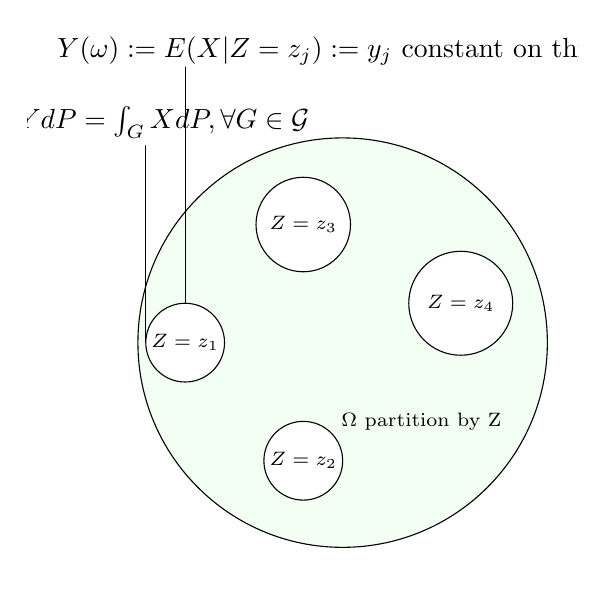
\begin{tikzpicture}[line cap=round,line join=round,>=triangle 45,x=1cm,y=1cm]
\clip(0,0) rectangle (7,7);
\draw[fill=green,fill opacity=0.05] (4,3) circle (2.6cm);
\draw[fill=white] (3.5,4.5) circle (0.6cm);
\draw[fill=white](3.5,1.5) circle (0.5cm);
\draw[fill=white](5.5,3.5) circle (0.66cm);
\draw[fill=white](2,3) circle (0.5cm);
\begin{scriptsize}
\draw[color=black] (2,3) node {$Z=z_1$};
\draw[color=black] (3.5,1.5) node {$Z=z_2$};
\draw[color=black] (3.5,4.5) node {$Z=z_3$};
\draw[color=black] (5.5,3.5) node {$Z=z_4$};
\draw[color=black] (5,2) node {$\Omega$ partition by Z};
\end{scriptsize}

\draw[-.](2,3.5) -- (2,6.5) ;
\draw[color=black] (3.8,6.7) node {$Y(\omega) := E(X|Z=z_j) := y_j$ constant on this};

\draw[-.](1.5,3) -- (1.5,5.5) ;
\draw[color=black] (1.5,5.8) node {$ \int_G YdP = \int_G XdP, \forall G \in \mathcal{G} $};

\end{tikzpicture}

\item $\mathcal{G}=\sigma(Z)$ generated by Z = sets on $\Omega \sucht \{Z \in B\}, B \in Borel$ = power set of the n ${Z=z_i}$ atoms = $2^n$ sets

\item $Y(\omega) := E(X|Z=z_j) := y_j$ constant on each $Z$ atom ie measurable

\item $\int_{Z=z_j}Y dP = y_jP(Z=z_j)\ =E(X|Z=z_j) P(Z=z_j) \\= \sum_i x_jP(X=x_i|Z=z_j)P(Z=z_j) = \sum_i x_jP(X=x_i,Z=z_j) = \int_{Z=z_j}X dP $

\item with $G_j={Z=z_j}$ we have $E(Y I_{G_j})=E(XI_{G_j})$ and then adding up all the $G_j$ we have $E(Y I_{G})=E(XI_{G})$ ie   \myhighlight {$$ \int_G YdP = \int_G XdP, \forall G \in \mathcal{G} $$}

\item \colorbox{green!10}{KOLMOGOROV:Conditional Expectation existence theorem} \\ given X such that:

\begin{enumerate}
\item $E|X| < \infty$ ie |X| integrable
\item $\mathcal{G} \subset \mathcal{F}$
\item $\Rightarrow \exists Y \sucht$
\begin{enumerate}
\item $Y \text{is } \mathcal{G}$-measurable
\item $E|Y| < \infty$ ie |Y| is integrable
\item $E(YI_G) = E(XI_G)\ \forall G \in \mathcal{G}$
\item any another such Y' will obey $P(Y=Y')=1$
\end{enumerate}
\end{enumerate}
\item \textbf{Proof outline} : 2 methods
\begin{enumerate}
\item proof method 1: Radon-Nikodym
\item proof method 2: Least-squares
\begin{enumerate}
\item prove a.s uniqueness of $E(X|\mathcal{G})$ (assuming it exists) : $E(Y;G)=E(Y';G)=E(X;G) \Rightarrow E(Y-Y';G)=0$. if $Y \neq Y'$ a.s then label Y,Y' such that $P(Y>Y')>0$. Now consider that $\{Y>Y'+ {1 \over n}\} \uparrow \{Y>Y'\}$, so for some $n$, $P(Y-Y'> {1\over n}) >0$, but that set $\{(Y-Y')> {1\over n}\} \in G$ since both G-meas. and $E(Y-Y';Y-Y'>{1 \over n})\ge {1 \over n} P(Y-Y' > {1 \over n}) >0 \Rightarrow$ contradiction

\item prove existence of $E(X|\mathcal{G})$ when $X \in L^2:=L^2(\Omega,\mathcal{F},\mathbb{P})$ : let $\mathcal{K}:=L^2(\Omega,\mathcal{G},\mathbb{P})$ with $\mathcal{G} \subset \mathcal{F}$. $\mathcal{K}$ complete in $L^2$-norm, take orthog.proj ie set $Y=\inf_{W \in L^2(\mathcal{K})} E [ {(X-W)}^2 ] $ which we know exists and is in $L^2$,and also it is orthog. proj ie $<X-Y,Z>=0\ \forall Z \in L^2(G)$, take $Z=1_G$ so that $E(X;G)=E(Y;G)\ \forall G$ ie the  l.s inf is as desired.

\item prove existence of $E(X|\mathcal{G})$ in general ie for $X \in L^1$ (since X integrable) : write $X=X^+-X^-$, prove if for $X^+$, choose bounded $bX_n$ (eg by truncation) such that $bX_n \uparrow X$, bounded so $bX_n \in L^2$, set $Y_n=E(bX_n|\mathcal{G})$, set $Y(\omega) := \limsup Y_n(\omega)$, then $Y \in m\mathcal{G}$ and $Y_n \uparrow Y \myright{MON-Prob} E(Y;\mathcal{G})=E(X;\mathcal{G}) \looparrowleft$ Recall :  \colorbox{green!10}{MON-Prob $  0 \le X_n \uparrow X \Rightarrow E(X_n) \uparrow E(X) \le \infty $}. So to finish using \colorbox{green!10}{Mon-Prob} we need to show $0 \le Y_n \uparrow$. 

\item so to finish we prove :  \colorbox{pink!30} { $U^+ \Rightarrow E(U^+|\mathcal{G}) \ge 0$} Proof: let $W=E(U^+|\mathcal{G})$, assume $P(W<0)>0$ then for some n $P(G:= W<-{1 \over n}) >0$ and $0 \le E(U^+;\mathcal{G}) = E(W;\mathcal{G}) < ={ {-1} \over n}$ contradiction;

\end{enumerate}
\end{enumerate}
\item $E(YI_G) = E(XI_G)\ \forall G \in \mathcal{G}$ 
\item Notation : such a Y is written $Y=E(X|\mathcal{G})$
\item Notation : $E(X|Z) \equiv E[X|\sigma(Z)] \equiv E(X|Z_1,Z_2,...)$
\item Notation : $E[X|\text{trivial sigma}]=E[X|\sigma(\emptyset,\Omega)] = E(X|\text{no information}) = E(X)$ ie $Y(\omega)=E(X|\mathcal{G})(\omega)=\text{constant } \forall \omega=E(X)$

\item conditional prob density: $f_{X|Z}(x|z) := \begin{cases} \frac{f_{X,Z}(x,z)}{f_Z(z)} \text{ if} f_Z(z) \neq 0 \\ 0\end{cases}$ 

\item Propertie of Conditional Expectations:
\begin{enumerate}

\item \colorbox{green!10}{ $E[E(X|\mathcal{G})]=E(X)$} \textbf{Proof}: $\looparrowleft E(Y;\Omega) \myeq{$\Omega \in \mathcal{G}$}  E(X;\Omega) = E(X)$

\item \colorbox{green!10}{ $X$ is  $\mathcal{G}$-measurable $\Rightarrow E(X|\mathcal{G})=XE(1|\mathcal{G})=X$ } \textbf{Proof}: $\looparrowleft$ use definition $Y := E(X|\mathcal{G})$ is such that $\int_{G \in \mathcal{G}} YdP = \int_{G \in \mathcal{G}} X dP$ and X will serve as this

\item \colorbox{green!10}{cLIN $E[aX+bY|\mathcal{G}] = a E[X|\mathcal{G}] + b E[Y|\mathcal{G}] $} \textbf{Proof} also use definition

\item \colorbox{green!10}{c+VE $X >= 0 \Rightarrow E(X|\mathcal{G}) \ge 0$} \textbf{Proof} : see proof for  \colorbox{pink!30} { $U^+ \Rightarrow E(U^+|\mathcal{G}) \ge 0$} above

\item \colorbox{green!10}{cMON+ $0 \le X_n \uparrow X  \Rightarrow E(X_n|\mathcal{G}) \uparrow E(X|\mathcal{G})$} \textbf{Proof}: same as above for Least-Squares

\item \colorbox{green!10}{cFATOU+ $0 \le X_n  \Rightarrow E(\liminf X_n|\mathcal{G}) \le \liminf E(X_n|\mathcal{G})$ a.s  } \textbf{Proof}: same as regular MON $\rightarrow$ FATOU proof

\item \colorbox{green!10}{cDOM $ |X_n(\omega)| \le V(\omega) \text{ with } E(V) <\infty \text{ and } X_n \longrightarrow X$} \\ \colorbox{green!10}{ $\Rightarrow E(X_n|\mathcal{G}) \longrightarrow E(X|\mathcal{G})$ a.s} \textbf{Proof}: same as regular FATOU $\rightarrow$ DOM proof

\item \colorbox{green!10}{cJENSEN $ convex : \mathbb{R} \mapsto \mathbb{R} \text{ with } E|convex(X)| < \infty$} \\ \colorbox{green!10}{ $ \Rightarrow convex(E(X|\mathcal{G})) \myle{Jensen} E(convex(X)|\mathcal{G}) $ } \textbf{Proof}: $convex \rightarrow$ continuous $\rightarrow convex(x)= \sup_n (a_nx+b_n)$ for some sequence $(a_n,b_n) \rightarrow \forall n\ c(x) \ge a_nx +b_n \myright{c+VE,cLIN} \forall n\ E[c(X)|\mathcal(G)] \ge \sup_n a_n E(X|\mathcal{G}) + b_n = c[E(X|\mathcal{(G)]}$  

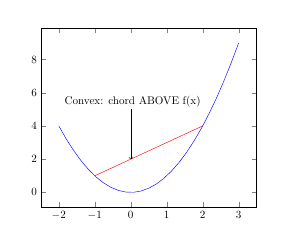
\begin{tikzpicture}[scale=0.4]
\begin{axis}
\addplot[domain=-2:3,blue] {x*x};
\addplot[domain=-1:2,red] {x+2};
\node[anchor=north] (source) at (axis cs:0,6){\text\ Convex: chord ABOVE f(x)};
\draw[->] (axis cs: 0,5) -- (axis cs: 0,2) ;
\end{axis}
\end{tikzpicture}

\item \colorbox{green!10}{cJENSEN Corollary $ {|| E(X|\mathcal{G}) ||}_p \le {||X||}_p $ } \textbf{Proof}: use $c(x)={|x|}^p, \forall p\ \ge 1$ in above and then take $\sqrt[p]{x} = {x}^{1 \over p}$ of both sides to get the  ${|| . ||}_p$

\item \colorbox{green!10}{TOWER $ E [ E (X | \mathcal{G}) | \mathcal{H}] = E (X | \mathcal{H})  $} Notation $E [ X | \mathcal{G} | \mathcal{H}] := E [ E(X | \mathcal{G}) | \mathcal{H}]$ \textbf{Proof} $\mathcal{H} \subset \mathcal{G}$ so (definition) $E(X|\mathcal{G})$ and $X$ are good candidates for $E(.|\mathcal{H})$

\item \colorbox{green!10}{TAKE OUT $G$ $\mathcal{G}$-measurable $\Rightarrow E(GX|\mathcal{G})=GE(X|\mathcal{G})$} \textbf{Proof}: for $Y=E(X|\mathcal{G})$, prove that $E(ZY;G)=E(ZX;G)$ for any $G \in \mathcal{G}$ and any $Z$ which is $\mathcal{G}$-measurable using 'standard machine' (ie starting with $Z={1}_G$, then linearity  for $Z \in {SimpleFun}^+(\Omega,\mathcal{G},\mathbb{P})$, then MON for $Z \in {(m\mathcal{G})}^+ $
	
\item \colorbox{green!10}{INDEPENDENCE $ \mathcal{H}$ indep of $\sigma(\sigma(X),\mathcal{G})$} \\ \colorbox{green!10}{ $\Rightarrow E[X|\sigma(\mathcal{G},\mathcal{H})]=E(X|\mathcal{G}$) } \textbf{Proof}: $ \mathcal{H}$ indep of $\sigma(\sigma(X),\mathcal{G})$ then $X1_G,H$ independent for $G \in \mathcal{G}$ so $E(X;G \cap H)=E[(X1_G)1_H] \myeq{indep} E(X1_G)E(1_H)=E(X1_G)P(H)$. Similarly for $Y=E(X|\mathcal{G})$ : $E[(Y1_G)(1_H)]=E(Y1_G)E(1_H)$ so $E(X;G \cap H)=E(Y;G \cap H)$ so the measures $\mu_1: F \mapsto E(X;F), \mu_2: F \mapsto E(Y;F)$ on $\sigma(\mathcal{G},\mathcal{H})$ agree on pi-system $G \cap H, G\in \mathcal{G}, H \in \mathcal{H} \Rightarrow$ agree  on $\sigma(\mathcal{G},\mathcal{H})$

\end{enumerate}

\item \colorbox{green!10}{Example} Compute $E(X_1| \frac{X_1+X_2+..+X_n}{n})$ with $X_1,...X_n$ iid same as $X$ : $E(X_1|S_n)=E(X_2|S_n)...=E(X_n|S_n)$ since $E(X_1;S_n \in B)=\int \int ... \int_{s_n \in B} x_1 \mu(dx1)\mu(dx2)...\mu(dxn)$ ; so $E(X_1|S_n)=E(X_2|S_n)...=E(X_n|S_n) = \frac{1}{n} E(X_1+...+X_n|S_n)=\frac{1}{n} E(S_n|S_n)=\frac{1}{n} S_n E(1|S_n)=\frac{S_n}{n}$

\end{itemize}

\section{Chapter 10 - Martingales II : Martingales }

\begin{itemize}

\item filtration : $\mathcal{F}_0 \subseteq \mathcal{F}_1 \subseteq ... \subseteq \mathcal{F}_n .. \subseteq \mathcal{F} $

\item  $\mathcal{F}_{\infty} := \sigma(\cup_n \mathcal{F}_n ) \subseteq \mathcal{F} $

\item normally $\mathcal{F}_n = \sigma (W_0,W_1,..,W_n)$ for some stoch. process $W$

\item information about $\omega$ at time n : $W_0(\omega),W_1(\omega),..,W_n(\omega)$

\item $X : \{X_i\}$ adapted to $\{\mathcal{F}_i\}$ if for each $n$, $X_n$ is $\mathcal{F}_n$-measurable

\item \colorbox{green!10}{Martingale definition} : X Martingale relative to $\mathcal{F}$
\begin{enumerate}
\item $X$ adapted to $\mathcal{F}$
\item $E{|X_n|} < \infty$ for all $n$
\item $E(X_n|{\mathcal{F}}_{n-1})=X_{n-1}$
\end{enumerate}

\item supermartingale decreases : $E(X_n|{\mathcal{F}}_{n-1}) \le X_{n-1}$
\item submartingale increases : $E(X_n|{\mathcal{F}}_{n-1}) \ge X_{n-1}$

\item Examples of martingales :
\begin{enumerate}

\item  \colorbox{green!10}{Sum of iid with $E(X_k)=0$ } ie $S_0:=0, S_n := X_1 + ...+ X_n$, $\mathcal{F}_{n}:= \sigma(X_1,X_2,...,X_n)$ then martingale \textbf{Proof:} $E(S_n|\mathcal{F}_{n-1})= E(S_{n-1}|\mathcal{F}_{n-1}) + E(X_n|\mathcal{F}_{n-1})=S_{n-1}+E(X_n)=S_{n-1}$ \\ \colorbox{red!10}{question}: $\lim S_n$ exists when ? [answer: Kolmogorov 3-series theorem]

\item  \colorbox{green!10}{Product of iid with $E(X_k)=1$ } ie $ M_n := X_1 ... X_n, E(X_i)=1, \myFF_n := \sigma(X_1,..,X_n)$ is martingale. \textbf{Proof:} $E(M_n|\myFF_{n-1}) = E(M_{n-1}X_n|\myFF_{n-1}) = M_{n-1} E(X_n|\myFF_{n-1}) \myeq{indep.} M_{n-1} E(X_n) = M_{n-1} $  \\ \colorbox{red!10}{question}: $\lim M_n$ exists when ? [answer: MCT : +ve rvs so $M_{\infty} := \lim M_n$ exists as] \\ \colorbox{red!10}{question}: $\lim E(M_{\infty})=1$ when ? [answer: Kakutani theorem on product martingale] 

\item  \colorbox{green!10} {Accumulating data : $\xi \in L^1 \rightarrow M_n := E(\xi|\myFF_n) $} is martingale \textbf{Proof}: $E(M_n|\myFF_{n-1}) = E(\xi|\myFF_n|\myFF_{n-1}) = E(\xi|\myFF_{n-1}) = M_{n-1} $ \\ \colorbox{red!10}{question}: $\lim M_n$  ? [answer: Levy upward theorem :$ M_n \rightarrow M_{\infty} := E(\xi|\myFF_{\infty})$ ]  \\ \colorbox{red!10}{question}: $\xi = E(\xi|\myFF_{\infty})$ when ? [answer : $\sum \frac{1}{c_k^2}$]

\end{enumerate}


\item game: $X_n-X_{n-1} , n \ge 1 $ = net win per unit stake i game n.

\item fair game: $E(X_n-X_{n-1} | \myFF_{n-1})=0$

\item previsible process: $C_n, n\ge 1$ is $\myFF_{n-1}$-measurable. $C_0$ does not exist.

\item $C_n$ stake on game n. 
\item  Winnings in  game n = $C_n(X_n-X_{n-1})$
\item  total Winnings up to game n := $Y_n := \sum_{1 \le k \le n}C_k(X_k-X_{k-1}) := {(C \bullet X)}_n$ [note: similar to $\int C dX$]

\item cannot beat the system
\begin{enumerate}

\item if X martingale, C bounded non-negative previsible ie $C_n(\omega) \ge 0, |C_n(\omega)| \le K $ then $(C \bullet X)$ martingale null at 0

\item if X martingale, C bounded previsible then $(C \bullet X)$ martingale null at 0

\item same if bounded $\Leftrightarrow L^2$ and X in $L^2$

\item \textbf{Proof:} $E(Y_n-Y_{n-1}|\myFF_{n-1}) = C_n E(X_n-X_{n-1}|\myFF_{n-1})$

\end{enumerate}

\item stopping time (A): $T_n$ stopping time if $ \{ T \le n \} = \{ \omega : T(\omega) \le n \} \in \myFF_{n}, \forall n \in [0,\infty]$ note $\infty$ is included

\item stopping time (B): same equivalent condition as $ \{ T = n \} = \{ \omega : T(\omega) = n \} \in \myFF_{n}, \forall n \in [0,\infty]$ \textbf{Proof}: if (A) then $ \{ T = n \} =  \{ T \le n \} \setminus \{ T \le n-1 \} \in \myFF_{n}$ if (B) $\{ T \le n \} \bigcup_{o \le k \le n} \{ T = n \} \in \myFF_{n} $ since $\myFF_{k} \subseteq \myFF_{n} , k \le n$

\item example of stopping time: time of first entry of A:= adapted process $\{A_n\}$ into B : $T = \inf \{n \ge 0 : A_n \in B\} $

\item example of NOT a stopping time: $T = \sup \{n \le 10 : A_n \in B\} $

\item stopped process : 
\begin{enumerate}
\item let X martingale
\item let T stopping time, 
\item let stake process $C^T$  be 0 after $T$ ie $C_n^{(T)} = I_{n \le T} =  \begin{cases} 1 \text{ if } n \le T(\omega) \\ 0 \text{after}\end{cases} $

\item wins process at time n : ${(C^{(T)} \bullet X)}_n= X_{T \wedge n} - X_0$ ie win is frozen after a while and dstays like that forver

\item let $X^T$ = process stopped (frozen) at T : $X_n^T(\omega) := X_{T(\omega) \wedge n}(\omega)$ $\looparrowleft \omega$ determines when to stop ad  also the value of X at that stopping point

\item then obviously $C^T \bullet X = X^T-X_0$ (wins are frozen after a while)

\item $C^{(T)}=0,1 \le 1, \ge 0$ so bounded and non-negative/ andprevisible because set to 0 once T is reached ie $\{ C_n{(T) = 0 }\} = \{T \le n-1\} \in \myFF_{n-1}$

\end{enumerate}

\item $X$ martingale, $T$ stopping time $\Rightarrow X^T$ martingale
\item in particular $E(X_{T \wedge n}) = E(X_0)$

\item \colorbox{red!20}{VERY IMPORTANT : Sometimes $E \left (X_{T \wedge n} \right ) \neq E(X_{T})$}
\item example : random walk on $\mathbb{Z^+}$ starting at 0 ,  first time hitting 1. Can prove $P(T < \infty)=1$. Then (as per above) $E(X_{T \wedge n})=E(X_0)=0$  but $E(X_{T})=1$ so $E (X_{T \wedge n} ) \neq E(X_{T})$

\item \colorbox{green!10}{Doobs optional stopping theorem} : gives conditions for $E (X_{T} ) = E(X_{0})$

\item \colorbox{green!10}{Doobs optional stopping theorem}
\begin{enumerate}
\item let T stopping time, X martingale
\item then IF one of the following holds, $E(X_T)=E(X_0)$ [not just $E(X_{T \wedge n} )$ ] :

\begin{enumerate}

\item T is certainly bounded ie $\exists N :  T(\omega) \le N $ \textbf{Proof:} set n=N in above

\item X is certainly bounded and T a.s finite ie $\exists K : |X_n(\omega)| \le K, \forall n, \forall \omega$ \textbf{Proof:} BDD so can use $n \rightarrow \infty$

\item $E(T)$ bounded aka integrable  and X increment bounded ie $E(T) < \infty$ and $\exists K : |X_n(\omega)-X_{n-1}(\omega) \le K|, \forall n, \forall \omega$ \textbf{Proof:} $ | X_{T \wedge n} - X_0|=| \sum_{k=1}^{T \wedge n} (X_k - X_{k-1})| \le KT$ and so can use DOM

\end{enumerate}

\end{enumerate}

\item \colorbox{green!10}{COROLLARY : Doobs optional stopping theorem}
\begin{enumerate}
\item let M martingale with bounded increment $K_1$
\item let C previsible with bound $K_2$
\item let T stopping time with $E(T) < \infty$
\end{enumerate}
then
\begin{enumerate}[resume]
\item $E {(C \bullet M)}_T = 0$ \textbf{Proof} $E {(C \bullet M)}_T = E {(C \bullet M)}_0 := 0$
\end{enumerate}

\item can use this for ABRACADABRA  problem and show $E(T)=26^{11} + 26^4 +26$

\item \colorbox{green!10}{When is $E(T) < \infty$ ?} : let stopping time T such that for some N and some $\epsilon$ : $P(T \le n + N| \myFF_n) > \epsilon \Rightarrow E(T) < \infty$

\item \colorbox{green!10}{hitting time for random walk}
\begin{enumerate}
\item let $P(X=+1)=P(X=-1)=\frac{1}{2}$
\item let $S_0 := 0, S_n := X_1 + \ldots + X_n$
\item let $T = \inf \{n : S_n =1 \}$
\item let $\myFF_{n} = \sigma(X_1, \ldots X_n) = \sigma(S_0,S_1, \ldots ,S_n)$
\item compute $E(e^{\theta X})= \frac{1}{2} ( e^{\theta} + e^{- \theta} ) = \cosh \theta$
\item so $E[(\sech \theta)e^{\theta X_n}]=1 , \forall n$
\item so (see prod of +ve martingales)  $M_n^{\theta}= {(\sech \theta)}^n e^{\theta S_n}$ is martingale

\item T stopping time so $EM_{T \wedge n}^{\theta}=1 = E[ {(\sech \theta)}^{T \wedge n} e^{\theta S_{T \wedge n}}]$

\item now let $\theta > 0$

\item $S_{T \wedge n} \le 1$ so $e^{\theta S_{T \wedge n}} \le e^{\theta}$, so $M_{T \wedge n}^{\theta} \le e^{\theta}$ ie bounded

\item note $ M_{T \wedge n}^{\theta} \rightarrow M_T^{\theta}$ as $ n \rightarrow \infty$

\item so can use BDD to let $ n \rightarrow \infty$ in $EM_{T \wedge n}^{\theta}=1$ to get $EM_{T }^{\theta}=1=E[ {(\sech \theta)}^T e^{\theta}]$

\item so $E[ {(\sech \theta)}^T ] =  e^{-\theta}$
\item so let $ \theta \downarrow 0$ then becasue $\sech \theta < 1$ we have $\begin{cases}  {(\sech \theta)}^T \uparrow 1 , \text{when} T < \infty \\ {(\sech \theta)}^T \uparrow 0 , \text{when} T = \infty \end{cases}$

\item both bounded so either MON or BDD gives $EI_{T < \infty} = 1 = P(T < \infty)$

\item let $\alpha = \sech \theta$ then from above $E[{(\sech \theta)}^T] = E(\alpha^T) = e^{-\theta}$

\item  then $E( {\alpha}^T) = \sum \alpha^{n} P(T=n) = e^{-\theta}=\frac{1-\sqrt{1-\alpha^2}}{\alpha} $

\item so find $P(T=k)$ by expansion

\end{enumerate}

\end{itemize}

\section{Chapter 11 - Martingales III : Martingale Convergence theorem }

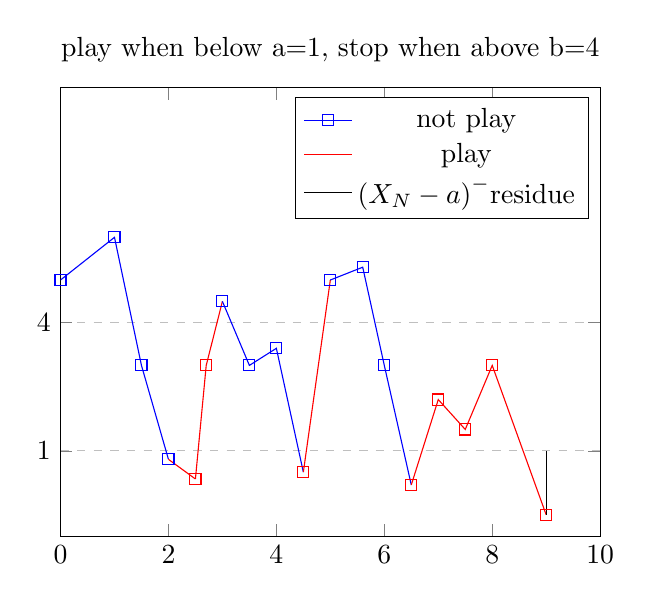
\begin{tikzpicture}

\begin{axis}[xmin=0,xmax=10,ymin=-1, ymax=9.5,ytick={1,4},ymajorgrids=true,grid style=dashed,
    title={play when below a=1, stop when above b=4},]

\addplot[color=blue,mark=square]coordinates {(0,5)(1,6)(1.5,3)(2,0.8)};
\addplot[color=red]coordinates {(2,0.8)(2.5,0.34)};
\addplot[color=red,mark=square]coordinates {(2.5,0.34)(2.7,3)(3,4.5)};
\addplot[color=blue,mark=square]coordinates {(3,4.5)(3.5,3)(4,3.4)(4.5,0.5)};
\addplot[color=red,mark=square]coordinates {(4.5,0.5)(5,5)};
\addplot[color=blue,mark=square]coordinates{(5,5)(5.6,5.3)(6,3)(6.5,0.2)};
\addplot[color=red,mark=square]coordinates{(6.5,0.2)(7,2.2)(7.5,1.5)(8,3)(9,-0.5)};
\addplot[color=black]coordinates{(9,-0.5)(9,1)};
\legend{not play,play,,,,,,${(X_N-a)}^{-}$residue}

\end{axis}
\end{tikzpicture}

\begin{itemize}
\item C previsible strategy: play when below a=1, stop when above b=4
\item $C_1 := I_{X_0<a}, C_n := I_{C_{n-1}=1} I_{X_{n-1} \le b} + I_{C_{n-1}=0} I_{X_{n-1} < a} \looparrowleft $ ie if previous = 1, then stay 1 while $\le b$, if previous = 0 then set to 1 when < a
\item let $Y = C \bullet X$ = gains process with that game. Y follows X when played, constant otherwise. $Y_0(\omega)=0$
\item number of upcrossings $U_N[a,b]$ = largest $k$ in partition that catches upcrossings = k in finest partition with $0 \le s_1 < t_1 \ldots s_{N-1} < t_{N-1} \le N$ that catches all the upcrossings ie $X(s_i)(\omega) < a,X(t_i)(\omega) > b$
\item $Y_N(\omega) \ge (b-a) U_N[a,b](\omega) - |X_N(\omega)-a| \looparrowleft $ upcrossings - last bit. Note -|first bit| = ignored
\item \colorbox{green!10}{Doob's upcrossing lemma} : $(b-a)EU_N[a,b] \le E[{(X_n-a)}^-]$ \textbf{Proof}  C previsible (see formula above), bounded (it is 0,1), +ve (same), and $Y=C \bullet X$, so Y supermartingale with $Y_0=0$ so $E(Y_N) \le 0$ then use above
\item corollary : let X supermartingale bounded in $L^1$ meaning $\sup_n E(|X_n|) < \infty$, and let $U_{\infty} \uparrow U_N[a,b]$, then 
\begin{enumerate}
\item \colorbox{green!10}{ $ \Rightarrow (b-a)EU_{\infty} \le |a| + \sup_n E(|X_n|) < \infty$} \textbf{Proof}: see above $(b-a) EU_N[a,b] \le |a| + E(|X_N|) \le |a| + \sup_n E(|X_n|)$ then use MON since all the functions positive.
\item so \colorbox{green!10}{ $P(U_{\infty}[a,b]=\infty)=0$ } \textbf{Proof} $EU_{\infty}[a,b]$ finite and U +ve and see sums of +ve rvs
\end{enumerate}
\item \colorbox{green!30}{Doob Martingale Convergence theorem} :  X supermartingale bounded in $L^1$ ie $\sup_n E(|X_n|) < \infty \Rightarrow X_{\infty} := \lim X_n := \limsup_n X_n $ exists, and $X_{\infty}$ is $\myFF_{\infty}$-measurable \textbf{Proof} $A := [\omega : X_n(\omega) \text{ does not converge to a limit in } [-\infty,+\infty] ] = [\omega : \liminf X_n(\omega) < \limsup X_n(\omega)] = \cup_{a,b \in \mathbb{Q}, a<b} [w : \liminf X_n(\omega) < a < b < \limsup X_n(\omega)] := \bigcup A_{a,b}$ but $A_{a,b} \subseteq [\omega : U_{\infty}[a,b](\omega)=\infty]$ so (above) $P(A_{a,b})=0$ so (countable $\bigcup$) $P(A)=0$ so $X_{\infty} := \lim X_n$ exists in $[-\infty,+\infty]$ a.s. But actually it is finite a.s because (FATOU) $E|X_{\infty}| = E(\liminf |X_n|) \le \liminf E |X_n| \le \sup_n E|X_n| < \infty$ so $P(X_{\infty})=1$

\item \colorbox{green!30}{WARNING} : yes $X_{\infty} := X_n$ exists but sometimes $E(X_{\infty}) \neq E(X_{n})$ - see branching process example

\item \colorbox{green!10}{Corollary} if X non-negative supermartingale  then $X_{\infty}:= \lim X_n$ exists a.s \textbf{Proof} bounded in $L^1$ since $E|X_n|=E(X_n) \le E(X_0)$

\end{itemize}
\section{Chapter 12 - Martingales III : Martingale Bounded in L2 }
\begin{itemize}
\item \textbf{Three series theorem, strong law of large numbers, Levy's extension of BC}

\item bounded in L2 (ie $\sup_n {||M_n||}_2 < \infty$) $\Rightarrow$ bounded in L1 (monotonicity of norms) and L2 easier because of formula $E(M_n^2) = E(M_0^2) + \sum_{k=1}^n E[{(M_k-M_{k-1})}^2]$ (proof below)

\item $M = (M_n : n \ge 0)$ martingale in $L^2$ ie $\forall n, E(M_n^2) < \infty$ so since martingale  $E(M_v|\myFF_{u})=M_u$ then $M_v - M_u \bot L^2(\myFF_{u})$ so $M_n = M_0 + \sum_{k=1}^n (M_k - M_{k-1})$ sum of orthogonal terms in L2 norm ie $E(M_n^2) = E(M_0^2) + \sum_{k=1}^n E[{(M_k-M_{k-1})}^2]$

\item M martingale in $L^2$ ie $M_n \in L^2$ then (a) $M \text{ bounded } \Leftrightarrow \sum E[{(M_k - M_{k-1})}^2] < \infty$ and then (b) $M_n \myright{$L^2$} M_{\infty}$ \textbf{Proof} (a) $E(M_n^2) = E(M_0^2) + \sum_{k=1}^n E[{(M_k-M_{k-1})}^2]$ so bounded one side $\Leftrightarrow$ bounded the other . (b) M bounded in  $L^2 \myright{monotonocity} \text{bounded in } L^1$ so $\myright{Doob convergence} \exists M_{\infty} := lim M_n$. Now pythagoras $E{(M_{n+r}-M_n)}^2 = \sum_{k=n+1}^{n+r} E[{(M_k-M_{k-1})}^2]$ , let $r \uparrow \infty$ and $E{(M_{\infty}-M_n)}^2 \myle{FATOU} \sum_{k \ge n+1} E[ {(M_k-M_{k-1})}^2]$ so $\lim_n E[{(M_{\infty}-M_n)}^2] =0$ so $M_n \myright{$L^2$} M_{\infty}$

\item \colorbox{green!10}{Sum of zero-mean RV with converging sum of Vars converges}
\item if $X_k$ such that $E(X_k)=0,\sigma_k^2 := \Var (x_k) < \infty$ then
\begin{enumerate}
\item $\sum \sigma_k^2 < \infty \Rightarrow \sum X_k $ converges a.s \textbf
\item Partial converse : if $\exists K \sucht |X_k(\omega)| \le K$ then  $\sum X_k $ converges a.s $\Rightarrow  \sum \sigma_k^2 < \infty$
\end{enumerate}

\item \textbf{Proof (1)} let $M_n=\sum_{k=1}^n X_k$.Now sum of IID RV $\Rightarrow$ martingale as we know already and $E{(M_k-M_{k-1})}^2=E(X_k^2)=\sigma_k^2$.Now since $E(M_n^2)=E(M_0^2) + \sum_{k=1} E{(M_k-M_{k-1})}^2 $ then $E(M_n^2)=\sum \sigma_k^2 := A_n$ , snd since $\sum \sigma_k^2 < \infty$ then M bounded in L2, so $\lim M_n$ exists as, 

\item \textbf{Proof (2)} $E [ {(M_k-M_{k-1})}^2 | \myFF_{k-1}] = E (X_k^2 | \myFF_{k-1}) \myeq{$X_k$ indep of $\myFF_{k-1}$} E(X_k^2) = \sigma_k^2$. Separately $M_{k-1}$ is $\myFF_{k-1}$-measurable so $\sigma_k^2=E(M_k^2|\myFF_{k-1}) - 2 M_{k-1}E(M_K|\myFF_{k-1}) + M_{k-1}^2 = E(M_k^2|\myFF_{k-1}) - M_{k-1}^2$ which shows that $N_n:=M_n^2-\sum_{k=1}^n \sigma_k^2$ is martingale. let $T:= \inf (r:|M_r|>c)$ then $N^T$ martingale so $EN_n^T=E{(M_n^T)}^2-EA_{T \wedge n}=EN_0=0$ with $A_n=\sum_{k=1}^n \sigma_k^2$, but $|M_T-M_{T-1}|=|X_T| \le K$ if T finite, so $|M_n^T| \le K+c$ so $ (\star) EA_{T \wedge n} \le {(K+c)}^2$. Now $\sum X_k$ sonverges $\Rightarrow $ partial sums bounded so for c big enough so $P(T=\infty)>0$ so from $(\star) \Rightarrow A_{\infty} := \sum \sigma_k < \infty$ 

\item random signs: $(a_n)$ seq. of real numbers and $\epsilon_n : P(\epsilon_n = \pm 1) = {1 \over 2}$  then from above:
\begin{enumerate}
\item $\sum \epsilon_n a_n$ converges $\Leftrightarrow \sum a_n^2 < \infty$

\item $\sum \epsilon_n a_n $ oscillates $\Leftrightarrow \sum a_n^2 = \infty$
\end{enumerate}

\item can prove above without need for zero-mean variable by symmetrising ie can prove: $X_n(\omega)$ bounded by K then $\sum X_k$ converges $\Rightarrow \sum E(X_k)$ converges and $\sum \Var (X_n) < \infty \looparrowleft$ no requirement for $E(X_k)=0$ \textbf{Proof sketch}: copy sample space $(\Omega^*,\myFF^*,\mathbb{P}^*)=(\Omega,\myFF,\mathbb{P}) \times (\Omega^@,\myFF^@,\mathbb{P}^@) $ and symmetrise with let $\omega^*=(\omega,\omega^@),X_k^*(\omega^*):= X_n(\omega),X_k^{*@}(\omega^*):=X_k^{@}(\omega^@) ,Z_k^*(\omega^*):=X_k^*(\omega^*)-X_k^{*@}(\omega^*)$ which now has 0-mean and is bounded because X is.

\item \colorbox{green!10}{KOLMOGOROV 3-SERIES} : $X_n$ iid sequence then $\sum_{k}X_k$ converges 
\begin{enumerate}
\item $\sum_{k}X_k$ converges
\end{enumerate}
\item $\Leftrightarrow$ all 3 hold for some K:
\begin{enumerate}
\item $\sum_n P(|X_n|>K) < \infty$
\item $\sum_n  E(X_n^K)$ converges
\item $\sum_n \Var(X_n^K) < \infty$
\item where $X_n^K(\omega) := \begin{cases} X_n(\omega) \text{ if } |X_n(\omega)| \le K \\ 0 \text{ otherwise} \end{cases} $
\end{enumerate}
\item \textbf{Proof} $\Leftarrow$\textbf{ (if)} So for some K the 3 properties hold. $\sum P(X_n \neq X_n^K) = P(|X_n|>K) < \infty$ so (BC1 -- see aside) $P(X_n = X_n^K$ for all but finitely many n - ie eventually)=1 

\item \colorbox{blue!10}{Recall BC1} : \colorbox{blue!10}{$ \sum P(E_n) < \infty \Rightarrow P(\limsup E_n) = P(E_n,\text{i.o})= 0 $} 

\item Aside: $(X_n\neq X_n^K,\text{ i.o})=\left\{\omega\::\: X_n(\omega)\neq X_n^K(\omega),\text{ i.o}\right) $ ie $=\left\{\omega\::\: \forall n\in\mathbb{N},\:\exists m>n\text{ with } X_m(\omega)\neq X_n^K(\omega)\right\}.=\left\{\omega\::\: \forall n\in\mathbb{N},\:\exists m>n\text{ with } X_m(\omega)\neq X_n^K(\omega)\right\}.$ The negation of $\forall n\in\mathbb{N},\:\exists m>n\text{ with } X_m(\omega)\neq X_n^K(\omega)$ is $\exists n\in\mathbb{N}\text{ such that }\forall m>n X_m(\omega)=X_n^K$. SO $\{\omega\::\: X_n(\omega)\neq X_n^K(\omega),\text{ i.o}\}^c=\{\omega\:;\:X_n(\omega)= X_n^K(\omega),\text{ eventually}\}$

\item Aside alternative proof :  $0 = P(\limsup \{X_n \neq X_n^K\}) = P(\cap_m \cup_{n > m} \{X_n \neq X_n^K\}) = 1 - P(\cup_m \cap_{n > m} \{X_n = X_n^K\}) \Rightarrow 1 = P(\liminf \{X_n = X_n^K\})$.

\item Anyway so $P(X_n = X_n^K$ for all but finitely many n - ie eventually)=1. So we only need to show that $\sum X_n^K$ converges a.s, and actually (property 2) , only need to show that $\sum Y_n^K$ converges where $Y_n^K := X_n^K - E(X_n^K)$ . Y is zero mean, finite var, so use (3) and earlier above.

\item \textbf{Proof} $\Rightarrow$ \textbf{(only if)} So suppose $\sum X_n$ converges a.s. Then $X_n \rightarrow 0$ a.s. Let any $K >0$ then $|X_n|>K$ for finitely many n, so (BC2) means prop (1) holds. [Recall BC2 :  $E_n$ independent , $\sum P(E_n) = \infty \Rightarrow P(\limsup E_n)=1$]. Since $X_n=X_n^K$ for all but finitely many n, $\sum X_n^K$ converges a.s. then use 'symmetrising' above.

\item \colorbox{green!10}{Cesaro}

\item \colorbox{green!10}{Kronecker}

\item \colorbox{green!10}{Strong law with variance constraint}

\item \colorbox{green!10}{Kolmogorov truncation lemma}

\item \colorbox{green!10}{Kolmogorov SLLN}

\end{itemize}
\section{Chapter 13 - Martingales IV : Uniform integrability }

\section{Chapter 14 - Martingales V : UI Martingales }

\section{Chapter 15 - Martingales VI : Examples }

\section{Chapter 16 - Characteristic functions I : Basics }

\section{Chapter 17 - Characteristic functions II : Weak convergence }

\section{Chapter 18 - Characteristic functions III : Central Limit theorem }

\end{spacing}
\end{multicols*}
\end{document}